\documentclass{article}
% Sorgt dafür, dass Überschriften wie "Inhaltsverzeichnis", "Glossar" usw. auf Deutsch sind und nicht auf Englisch
\usepackage[ngerman]{babel}
% Wird benötigt, um Grafiken einzufügen
\usepackage{graphicx}

% Wird benötigt, um selbst Grafiken zeichnen zu können
\usepackage{tikz}

% Wird für Tabellen benötigt
\usepackage{booktabs}

% Wird benötigt, um bestimmte Symbole in Abbildungen zu zeichnen
\usepackage{amsmath}
\usepackage{amssymb}


% Wird benötigt, um Wikel zeichnen zu können
\usetikzlibrary{angles, quotes}


\graphicspath{ {./Bilder/} }

% Wird zur besseren Positionierung von Grafiken oder Tabellen gebraucht
\usepackage{float}



\usepackage[utf8]{inputenc}

% Wird für das Literaturverzeichnis benötigt
\usepackage[backend=biber,style=numeric]{biblatex}
% Fügt das Literaturverzeichnis hinzu
\addbibresource{literatur.bib}
\makeindex

% Dieses Paket wird benötigt, um automatisch ein Abkürzungsverzeichnis zu generieren
\usepackage{glossaries}
\makeglossaries

\newglossaryentry{latex}
{
    name=latex,
    description={Is a markup language specially suited for scientific documents}
}

\newglossaryentry{Spawnpunkt}
{
    name=Spawnpunkt,
    description={Bezeichnet eine 2D oder 3D Koordinate in einer Simulationsumgebung oder in einem Videospiel, an welchem virtuelle Objekte instanziiert werden}
}



\title{Implementierung eines Eye-Tracking Systems in den Fahrsimulator der Hochschule Karlsruhe}

\author{\Large Projektarbeit \\ \\ Jonas Verleger, Lenard Haas}
\date{... April 2025}

\newacronym{api}{API}{Application Programming Interface}

\newacronym{rgb}{RGB}{Rot, Grün, Blau (Farbraum)}

\newacronym{id}{ID}{Identifikationsnummer}

\newacronym{sdk}{SDK}{Software Development Kit}


\begin{document}
  
\maketitle
\newpage
\tableofcontents
\newpage



\section{Einführung}
\setlength{\parskip}{6pt plus 2pt minus 1pt}

Das menschliche Fahrverhalten ist bedingt durch die Vielzahl der möglichen Situationen und Reaktionen im Straßenverkehr höchst komplex. Eine Analyse dessen ist somit nur durch initiale Vereinfachungen in einem Modell möglich oder durch eine realistische Simulation mir realen Fahrern. Für den zweiten Ansatz entwickelt das Institut für Energieeffiziente Mobilität (IEEM) ein Simulationsframework, welches mit unterschiedlichen Bewegungsmethoden (Auto, Fahrrad, Gehen) und in unterschiedlicher Realitätsnähe genutzt werden kann.

Als Softwarebasis dient das Open-Source-Projekt CARLA. CARLA ermöglicht es, verschiedene Verkehrsszenarien und Wetterbedingungen einzustellen. Die Analyse des menschlichen Verhaltens im Straßenverkehr kann somit ohne Gefahren und in verschiedensten simulierten Szenarien erfolgen. Die Server-Client Struktur von CARLA lässt ebenso mehrere Probanden in demselben Verkehrsszenario zu. So können menschliche Interaktionen realitätsnah nachgebildet werden.

Für die Analyse des Fahrverhaltens wird mindestens die Auswertung der Fahrzeugdaten (z. B.: der zurückgelegte Weg, einwirkende Kräfte) benötigt. Für eine genauere Analyse eignen sich zudem die Fahrerentscheidungen. Diese können einen Einblick geben, ob ein Fahrmanöver aus Reflex erfolgt ist oder ob es eine bewusste Entscheidung gewesen ist. Ein einfacher Weg Fahrerentscheidungen zu erfassen, ist es, dass nach einem Fahrversuch ein Fragebogen beantwortet wird. Weiterführend bietet es sich an Echtzeitdaten des Probanden aufzuzeichnen.

Eine große Rolle für das Treffen von Entscheidungen spielt die Sicht. Hierdurch wird deutlich, was die Probanden bei der Testfahrt sehen, worauf diese sich konzentrieren und welchen Fahrweg sie nehmen werden. Für die Datenerhebung der Sicht eignet sich ein sogenannter Eye-Tracker.

\subsection{Zielsetzung}

Im Rahmen dieser Projektarbeit soll ein kamerabasierter Eye-Tracker entwickelt werden, der in die CARLA Simulationsumgebung integriert werden kann.

Dazu werden mögliche Eye-Tracker auf die Anwendbarkeit und Integration in CARLA analysiert. Ebenfalls wird eine Simulation in CARLA erstellt, um den Eye-Tracker zu testen. Weitere Vorgaben sind die Projektion des Blickpunktes auf die Leinwand und eine Ausgabe der aufgezeichneten Daten.

\subsection{Lösungsansatz}

Damit die gesetzten Ziele erreicht werden, werden zuerst die Grundlagen von Eye-Trackern und der CARLA-Simulationsumgebung erarbeitet. Für die Integration in das Gesamtsystem wird ein objektorientierter Python Code entwickelt. Der Code soll den Blickpunkt des Probanden als Pixel ausgeben und mit CARLA austauschen können. Ebenfalls wird die benötigte Rechenleistung minimiert. Die Ausgabe der erhobenen Daten erfolgt in Echtzeit über ein Fenster und wird im .csv-Format abgespeichert.

\section{Eye Tracker}

In diesem Kapitel wird ein grober technischer Einblick in die Funktionen eines Eye-Trackers geliefert. Daraufhin wird im Sinne des zeitlichen Rahmens des Projektes eine Marktanalyse durchgeführt, um verfügbare Eye-Tracker auf derer Anwendbarkeit, Integration in CARLA und Kosten zu untersuchen.

\subsection{Technische Grundlagen}

Die Hardwarevoraussetzungen für einen Eye-Tracker belaufen sich auf eine Kamera, Lichtquellen und einen Computer. Für die Kamera genügt eine einfache Webcam. Die Genauigkeit des Eye-Trackers kann gesteigert werden, indem eine hochauflösende und schnell aufzeichnende Kamera genutzt wird. Besonders eignet sich eine Infrarotkamera, weil im Nachgang in der Bildverarbeitung eine Graustufen Konvertierung durchgeführt wird. Zudem ermöglicht eine hohe Aufzeichnungsfrequenz der Kamera die Analyse von schnellen Blicksprüngen.

Die Genauigkeit des Eye-Trackers kann ebenso durch gute Beleuchtung vom Gesicht des Probanden verbessert werden. Um dabei nicht für ein Blenden zu sorgen, kann eine Infrarotquelle genutzt werden. Das erfordert zwingend eine Infrarotkamera, um den Effekt der besseren Beleuchtung ausnutzen zu können. Weiterreichend muss der Computer, welcher die Bildverarbeitung durchführt, ausreichend Rechenleistung liefern. Dadurch können Berechnung und Analyse in einer höheren Frequenz erfolgen, wodurch die Genauigkeit ebenfalls gesteigert werden kann.

Um die Pupillen zu erkennen, wird das aufgezeichnete Kamerabild vorverarbeitet. Die Graustufen Konvertierung sorgt für eine Vereinfachung der Bildverarbeitung, indem Farbinformationen entfernt werden. Optional kann eine Rauschfilterung implementiert werden. Bei fordernden Hintergründen oder unzureichender Belichtung sorgt die Filterung für eine Verbesserung der Ergebnisse. Als letzten Schritt der Vorverarbeitung wird der Kontrast verstärkt, sodass Merkmale besser erkannt werden können.

\textcolor{red}{BILD mit Vorverarbeitungsschritten}

Mit dem vorverarbeiteten Bild erfolgt die Merkmalerkennung. Die Pupillen können mittels verschiedener Verfahren erkannt werden. Ein einfacher, aber ungenauer Weg ist das Schwellenwertverfahren. Hierbei wird ein fester Wert und Ort deklariert, in welchem die Pupillen liegen können. Bei falscher Parametrisierung kann es somit zur falschen Erkennung kommen. Die Hough-Transformation ermöglicht eine robustere Erkennung, da Kreise erkannt werden können \textcolor{red}{QUELLE}. Maschinelles Lernen kann ebenso genutzt werden, um ein breiteres Spektrum an möglichen Pupillenpositionen im Kamerabild abzudecken. Durch maschinelles Lernen können weitergehend kompliziertere Situationen bei der Bildaufzeichnung geregelt werden.

Bei Nutzung einer Infrarotkamera kann die Reflektion des Infrarotlichtes auf der Hornhautoberfläche des Auge identifiziert werden. Diese Reflektion, genannt Glint, sorgt für eine Trennung der Pupillenposition und dem Kameraaufzeichnungswinkel \textcolor{red}{QUELLE}. Optional lässt sich die Augenumrandung zur zusätzlichen Orientierung mit analysieren.

\textcolor{red}{BILD mit Merkmalen}

Die Berechnung der Blickrichtung auf den Bildschirm erfolgt durch geometrische Modelle. Optional kann maschinelles Lernen eingesetzt werden. Für die Abbildung der Blickposition wird eine Kalibrierung benötigt. Diese erfolgt zu Beginn des Aufzeichnungsprozesses über fest definierte Punkte auf dem Bildschirm. Dadurch wird die Pupillenposition einer Bildschirmkoordinate zugeordnet. Mithilfe geometrischer Modelle wird eine Funktion berechnet, die basierend auf der Kalibrierung alle Bildschirmpunkte abdeckt. Die Genauigkeit kann über die Glint-Messung verbessert werden. Hierdurch lässt sich ein Vektor zwischen dem Pupillenmittelpunkt und der Glint-Position berechnen. Die Veränderung des Vektors nach der Kalibrierung hilft der Abbildung des Blickes auf dem Bildschirm.

Der fertige Eye-Tracker gibt die berechnete Blickposition als x-/y-Koordinate für den Bildschirm aus. Optional können weitere Funktionen hinzugefügt werden, wie beispielsweise das Zeichnen des Blickpunktes auf den Bildschirm, die zeitliche Analyse von Blickpunkten und die Abspeicherung der gemessenen Werte.

\subsection{Marktanalyse} 

Da die Entwicklung eines eigenen Eye-Tracking Algorithmus den zeitlichen Rahmen der Projektarbeit übersteigt, wird eine Marktanalyse von Eye-Trackern durchgeführt.

Ein erster Softwarekandidat ist ein Open Source Tracking Projekt auf GitHub \textcolor{red}{QUELLE}. Die Ausgabe dieses Trackers ist in Abbildung \ref{fig:old_tracker_face_gaze_webcam} zu erkennen. Das System orientiert sich hauptsächlich an den Augen und der Nase der Testperson. Dadurch kann es recht genau bestimmen, in welche Richtung der Kopf einer betrachteten Person geneigt ist. Zudem kann die Software das Blinzeln der Augen erkennen. Hierdurch kann theoretisch eine Analyse durchgeführt werden, welche die Reaktionszeit mit einem Blinzeln in Relation setzt. In diesem Projekt fällt ein solcher Betrachtungswinkel weg.

Die Software schätzt nicht die Blickposition der Testperson auf dem Bildschirm, sondern gibt nur an, in welcher Lage sich der Kopf befindet. Diese Daten könnten aber als Grundlage dienen für eine Weiterentwicklung. Da allerdings nur die Ausrichtung des Gesichts und nicht der Pupillen in die Ausgabe einfließt, erwarten wir keine besonders genauen Ergebnisse durch diese Herangehensweise.

\begin{figure}[h!]
\begin{center}
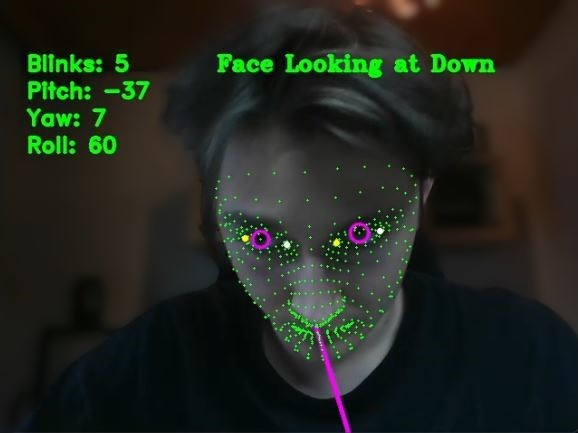
\includegraphics[scale=0.4]{old_tracker_face_gaze_webcam}
\caption{Ausgabe des Face-Gaze-Trackers, Quelle: \cite{lit_code_github_facegazetracker}} \label{fig:old_tracker_face_gaze_webcam}
\end{center}
\end{figure}

Eine weitere Option stellt das open source Projekt eyegaze Tracker dar. Diese Software erfasst nicht die Gesichtsausrichtung, sondern die Pupillen. Dadurch kann sie Aussagen über die grobe Blickrichtung treffen. So wie in Abbildung \ref{fig:old_tracker_eyegaze_webcam} zu erkennen, kann bspw. die Aussage getroffen werden, dass die Testperson nach links schaut. Auch hier wird keine Blickposition auf dem Bildschirm geschätzt. Allerdings werden die Pupillen erfasst und die grobe Blickrichtung bestimmt. Die Blickposition kann gegebenenfalls mit den vorhandenen Daten durch eine Weiterentwicklung des vorhandenen open source Codes bestimmt werden. Dies würde allerdings sehr viel Entwicklungsaufwand bedeuten. 

\begin{figure}[h!]
\begin{center}
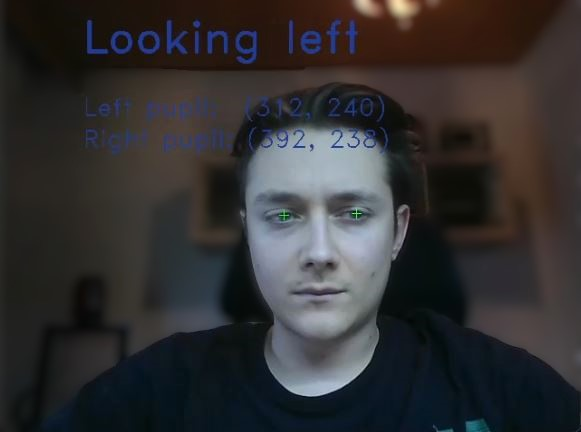
\includegraphics[scale=0.4]{old_tracker_eyegaze_webcam}
\caption{Ausgabe des Eyegaze-Trackers, Quelle: \cite{lit_code_github_gazetracking}} \label{fig:old_tracker_eyegaze_webcam}
\end{center}
\end{figure}

Neben den oben genannten Projekten wurden auch noch einige weitere auf ihre Einsetzbarkeit in diesem Projekt untersucht. Diese hatten größtenteils ähnliche Eigenschaften und Einschränkungen. Es wurde sich nach viel Recherche und Experimenten für den Beam Eye Tracker von Eyeware Tech entschieden. Dieser hat unsere Anforderungen grundlegend erfüllt und soll als Basis für die weitere Entwicklung dienen.

\subsection{Beam Eye Tracker}

Der Beam Eye Tracker ist für Gaming-Anwendungen und einfacher Nutzung entwickelt. Mithilfe einer einfachen Webcam erzeugt Beam die Blickposition auf dem Bildschirm. Ebenso verfügt das Programm über eine Kopfpositionserkennung relativ zum Bildschirm. Durch die Funktion "Gaming Erweiterungen" teilt Beam die Trackingdaten mit anderen Programmen. Diese Schnittstelle ermöglicht die Nutzung der Trackingdaten für eigene Programme via des Beam Software Development Kit.

\textcolor{red}{BILD vom Beam UI}

Die Beam API kann über die Programmiersprachen C++, C, C\# und Python angesprochen werden. Im Rahmen dieser Projektarbeit wird die Python Integration genutzt. Verschiedene Klassen in der API ermöglichen eine individuelle Nutzung des eigenen Programmes. Relevant für diese Projektarbeit ist die Klasse \glqq{}screen\_gaze\_info\grqq{}. Diese beinhaltet die x- und y- Koordinaten und die Angaben, ob die Augen erkannt werden und wie sicher diese Erkennung ist.

Durch die einfache Nutzung der Beam SDK und dem Preis von 29,99 € des Eye-Trackers fiel die Entscheidung, diesen für das Projekt zu nutzen. In Rücksprache mit den Beam Entwicklern wurde der Beam Eye Tracker für dieses Projekt kostenlos zur Verfügung gestellt.

\section{Implementierung Eye Tracker}

\subsection{Einrichtung im Fahrsimulator}

Eyeware Tech setzt bei ihrem Beam Eye Tracker auf einfache Hardware. Dieser arbeitet mit einer einfachen USB Webcam oder mit einem an den Computer angeschlossenen Smartphone-Kamera. Damit der Einsatz des Eye Trackers im Fahrsimulator gelingt, müssen einige Punkte beachtet werden. 

Die Positionierung der Kamera ist sehr wichtig. Diese soll lauf Eyeware Tech mittig zum Bildschirm ausgerichtet sein \cite{lit_software_beam_eyetracker}. Die Sitzposition der Testperson hingegen muss nicht mittig zur Kamera sein. Die Testperson kann auch relativ zur Kamera weiter links oder weiter rechts sitzen.
In den Eye Tracker Einstellungen muss auch die Kameraposition und der Neigungswinkel korrekt eingestellt werden. Die besten Ergebnisse konnten erzielt werden, als die Kamera im Fahrsimulator mittig auf dem Display in der Mitte des Armaturenbretts angebracht war. Die Kameraposition wurde im Eye Tracker als "unten" und mit einem Neigungswinkel von 0° angegeben.

Grundlage für gute Ergebnisse ist es die Kalibrierung, welche der Beam Eye Tracker integriert hat, vor jeder Sitzung im Fahrsimulator durchzuführen. Besonders wenn mehrere Personen nacheinander fahren, die sich von ihrer Körpergröße stark unterscheiden. Die in den Beam Eye Tracker integrierte Kalibrierung besteht aus fünf Punkten, die nacheinander auf der Leinwand erscheinen. Vier Punkte werden dabei in die vier Ecken der Leinwand positioniert. Der fünfte Punkt befindet sich in der Mitte der Leinwand. Während der Kalibrierung muss die Testperson nacheinander auf diese Punkte schauen. Sofern die Testperson einen Punkt fest fokussiert hat, klickt sie mit der Maus auf diesen Punkt. Der Eye Tracker verknüpft dann die aktuelle Blickposition mit den Koordinaten des Punktes auf der Leinwand. Nach diesem Prinzip kalibriert sich der Eye Tracker selbst und verknüpft die Position der Pupillen mit einer Position auf der Leinwand.

Da die Leinwand sehr groß ist und das Kalibrierungsfenster des Eye Trackers nicht verkleinert werden kann, befinden sich die Kalibrierungspunkte teilweise so weit in den Ecken, dass sie vor allem unten nicht mehr auf der Leinwand angezeigt werden. Das macht es schwer sie anzuklicken. Außerdem sollten während der Kalibrierung keine großen Kopfbewegungen gemacht werden. Es hat sich in Experimenten gezeigt, dass das die Tracking Genauigkeit verringern kann. Da die Punkte durch die breite Leinwand aber außerhalb des Sichtfelds der Testperson liegen, muss diese zwangsweise eine Kopfbewegung machen. 

Eine Herangehensweise um diese Probleme zu umgehen ist es, die Kalibrierung immer zu zweit durchzuführen. Die Testperson ist dafür verantwortlich auf die Kalibrierungspunkte zu schauen und die zweite Person klickt auf diese mit der Maus. Da die Punkte teilweise außerhalb des Sichtfeldes liegen und die Testperson den Kopf nicht zu sehr bewegen sollte, ist es am besten, wenn diese nicht direkt auf den jeweiligen Punkt schaut, sondern leicht daneben. Wenn der Punkt bspw. unten rechts im Eck erscheint, dann schaut die Testperson bei der Kalibrierung etwas weiter nach links. Zum einen wird dadurch die Kalibrierung insgesamt verbessert, da der Kopf nicht bewegt werden muss. Zusätzlich wird dadurch ein Fehler leicht abgeschwächt, welcher durch die Krümmung der Leinwand entsteht.
Zwischenzeitlich wurde im Rahmen dieser Projektarbeit auch der Ansatz einer eigenen Kalibrierung verfolgt. Diese hat vorausgesetzt, dass der Eye Tracker bereits einmal sehr grob mit dem integrierten Kalibrierungsfenster von Beam kalibriert wurde. Bei jedem Start des Programms wurde das selbst erstellte Kalibrierungsfenster geöffnet. Dieses hat nach demselben Prinzip wie das im Beam Eye Tracker integrierte Kalibrierungsfenster gearbeitet. Allerdings war das selbst entwickelte Kalibrierungsfenster in seiner Größe anpassbar. Dadurch wurden die Punkte im Sichtfeld der Testperson angezeigt und nicht an den Rändern der Leinwand. Eine schematische Abbildung des Kalibrierungsgfensters ist in Abbildung \ref{fig:eigenes_kalibrierungsfenster} zu sehen. In der Realität hatte das Fenster einen weißen Hintergrund, um die Lichtverhältnisse relativ zum Beam Kalibrierungsfenster zu verbessern. Die Ergebnisse der Kalibrierung wurden anschließend verwendet, um die Rohdaten des Eye Trackers mit diesen zu transformieren, damit die Kalibrierung Einfluss auf die Schätzwerte der Blickposition nimmt. Die daraus resultierten Ergebnisse wiesen allerdings keine wirkliche Verbesserung auf. Es wird daher empfohlen die integrierte Standard-Kalibrierung des Eye Trackers zu verwenden. Der Code für die selbst entwickelte Kalibrierung ist allerdings weiterhin in auskommentierter Form vorhanden und kann bei Bedarf wieder reaktiviert und weiterentwickelt werden. 

\begin{figure}[h]
	\begin{center}
    \begin{tikzpicture}[scale=0.9]
        % Fensterhintergrund
        \draw[fill=gray!20] (0,0) rectangle (8,6);

        % Fensterleiste mit Min, Max, Schließen
        \draw[fill=gray!40] (0,6) rectangle (8,6.5);
        \draw[fill=black] (6.8,6.2) rectangle (7.1,6.4); % Minimieren
        \draw[fill=black] (7.2,6.2) rectangle (7.5,6.4); % Maximieren
        \draw[fill=red] (7.6,6.2) rectangle (7.9,6.4); % Schließen
        \node at (6.95,6.3) {\textcolor{white}{\scalebox{0.7}{$-$}}};
        \node at (7.35,6.3) {\textcolor{white}{\scalebox{0.7}{$\square$}}};
        \node at (7.75,6.3) {\textcolor{white}{\scalebox{0.7}{X}}};

        % Kalibrierungsknöpfe
        \draw[fill=blue!40] (0.3,0.5) rectangle (2.2,2); % Unten links
        \draw[fill=blue!40] (5.8,0.5) rectangle (7.7,2); % Unten rechts
        \draw[fill=blue!40] (0.3,4) rectangle (2.2,5.5); % Oben links
        \draw[fill=blue!40] (5.8,4) rectangle (7.7,5.5); % Oben rechts
        \draw[fill=blue!40] (3.05,2.25) rectangle (4.95,3.75); % Mitte

        % Text auf den Knöpfen
        \node at (1.25,1.25) {\small \textbf{kalibrieren}};
        \node at (6.75,1.25) {\small \textbf{kalibrieren}};
        \node at (1.25,4.75) {\small \textbf{kalibrieren}};
        \node at (6.75,4.75) {\small \textbf{kalibrieren}};
        \node at (4,3) {\small \textbf{kalibrieren}};
    \end{tikzpicture}
	\end{center}
	\caption{Schematische Darstellung des selbst entwickelten Kalibrierungsfensters}\label{fig:eigenes_kalibrierungsfenster}
\end{figure}


Während der Kalibrierung und der gesamten Verwendung des Eye Tracking Systems darf nur die Testperson im Fahrsimulator sitzen. Eine zweite Person würde das Tracking System beeinflussen, da nicht selektiert werden kann, welche Augen getrackt werden sollen und welche nicht. In Zukunft muss hier eine Art Scheuklappe eingebaut werden, um dieses Problem zu lösen. 

Ein weiterer wichtiger Faktor ist die Beleuchtung im Fahrsimulator. Das Kalibrierungsfenster des Beam Eye Trackers hat einen schwarzen Hintergrund. Wenn keine externe Lichtquelle verwendet wird, dann ist es definitiv zu dunkel, als dass eine ordentliche Kalibrierung stattfinden könnte. Selbst wenn während der Kalibrierung gute Lichtverhältnisse herrschen, reicht die Helligkeit der Leinwand während des Fahrens oft nicht aus, um verlässliche Ergebnisse zu liefern. Es konnte eine starke Verbesserung der Trackingqualität erzielt werden, nachdem im Fahrsimulator eine externe Lichtquelle während der gesamten Kalibrierung und der gesamten Fahrzeit eingesetzt wurde. 
Neben externen Mitteln, um die Lichtverhältnisse zu verbessern, können auch in der Windows Kamera App Anpassungen vorgenommen werden. Dazu muss in den Einstellungen der Kamera App unter "Kameraeinstellungen" die Option "Erweiterte Steuerelemente für Fotos und Videos" aktiviert werden. Dadurch wird ein Helligkeitsregler verfügbar, der die Helligkeit des Kamerabildes systemweit verändert. Je nach aktuellen Lichtverhältnissen kann ein Erhöhen oder Verringern der Bildhelligkeit den Kontrast der Pupillen relativ zur Umgebung verbessern. Bei der Wahl der Kamera sollte eine Kamera verwendet werden, welche eine Auflösung von mindestens 1920x1080 besitzt. 

\begin{figure}[h!]
\begin{center}
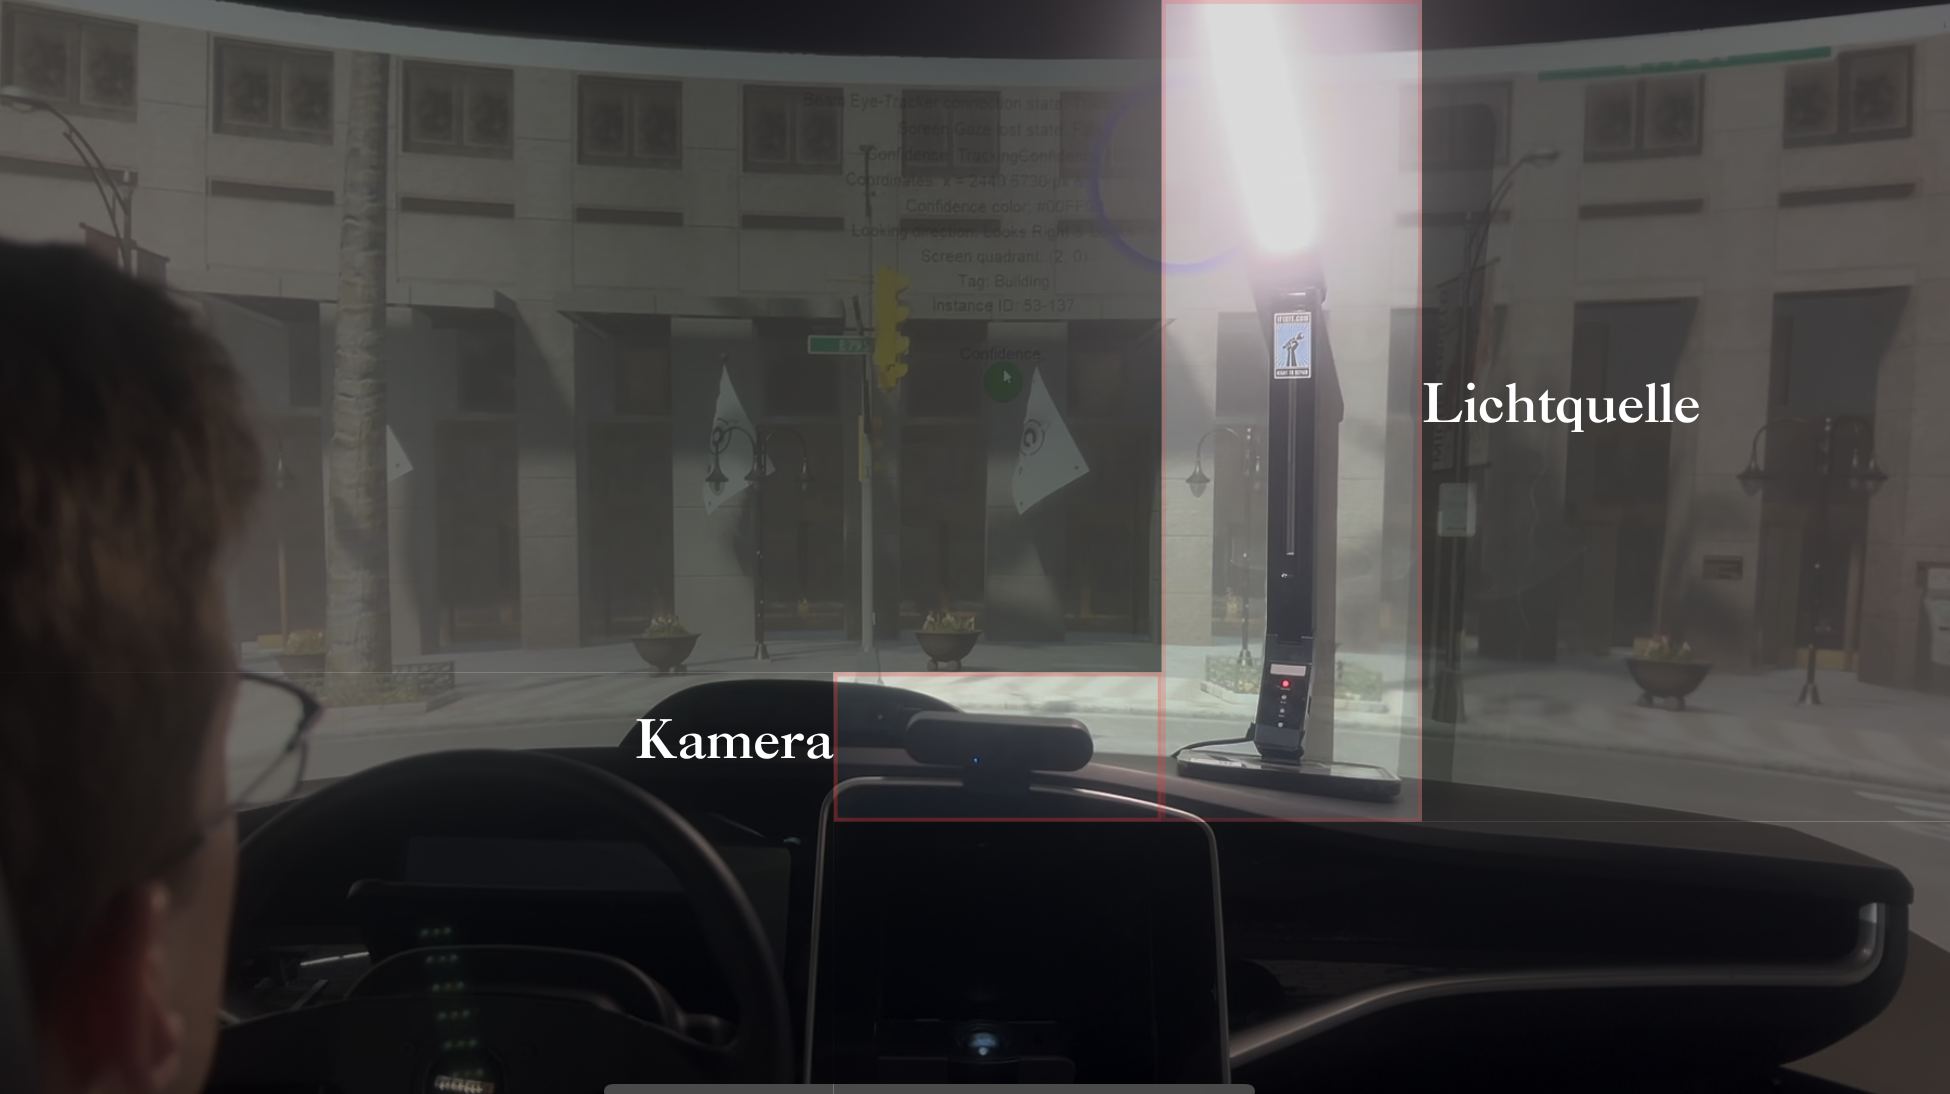
\includegraphics[scale=0.19]{camera_position}
\caption{Positionierung von Kamera und externer Lichtquelle, Quelle: \cite{lit_software_canva}} \label{fig:camera_position}
\end{center}
\end{figure}


In Abbildung \ref{fig:camera_position} sind die Kameraposition und die externe Lichtquelle aufgebaut im Fahrsimulator zu erkennen. Licht und Kamera sollten zu einem späteren Zeitpunkt noch besser in das System integriert werden. Zu Testzwecken hat der Aufbau allerdings gute Ergebnisse geliefert. 


  

\subsection{Beam Eye Tracker SDK}
Eyewear Tech bietet beim Kauf des Beam Eye Tracker das Beam-Software Development Kit (\acrshort{sdk}) an. Das \acrshort{sdk} ermöglicht es die Ausgabe des Eye Trackers in selbst geschriebenen Anwendungen zu verwenden \cite{lit_website_beam_sdk_documentation}.
Auf der Website des Beam \acrshort{sdk} wird in Python geschriebener Beispielcode zur Verfügung gestellt. In diesem Code werden die nötigen Schritte für eine Verbindung mit der API des Eye Trackers durchgeführt. Der Code wurde auch als Grundlage für die Implementierung des Eye Trackers in das von uns geschriebene Programm verwendet \cite{lit_code_beam_sdk}.


\begin{figure}[h!]
\begin{center}
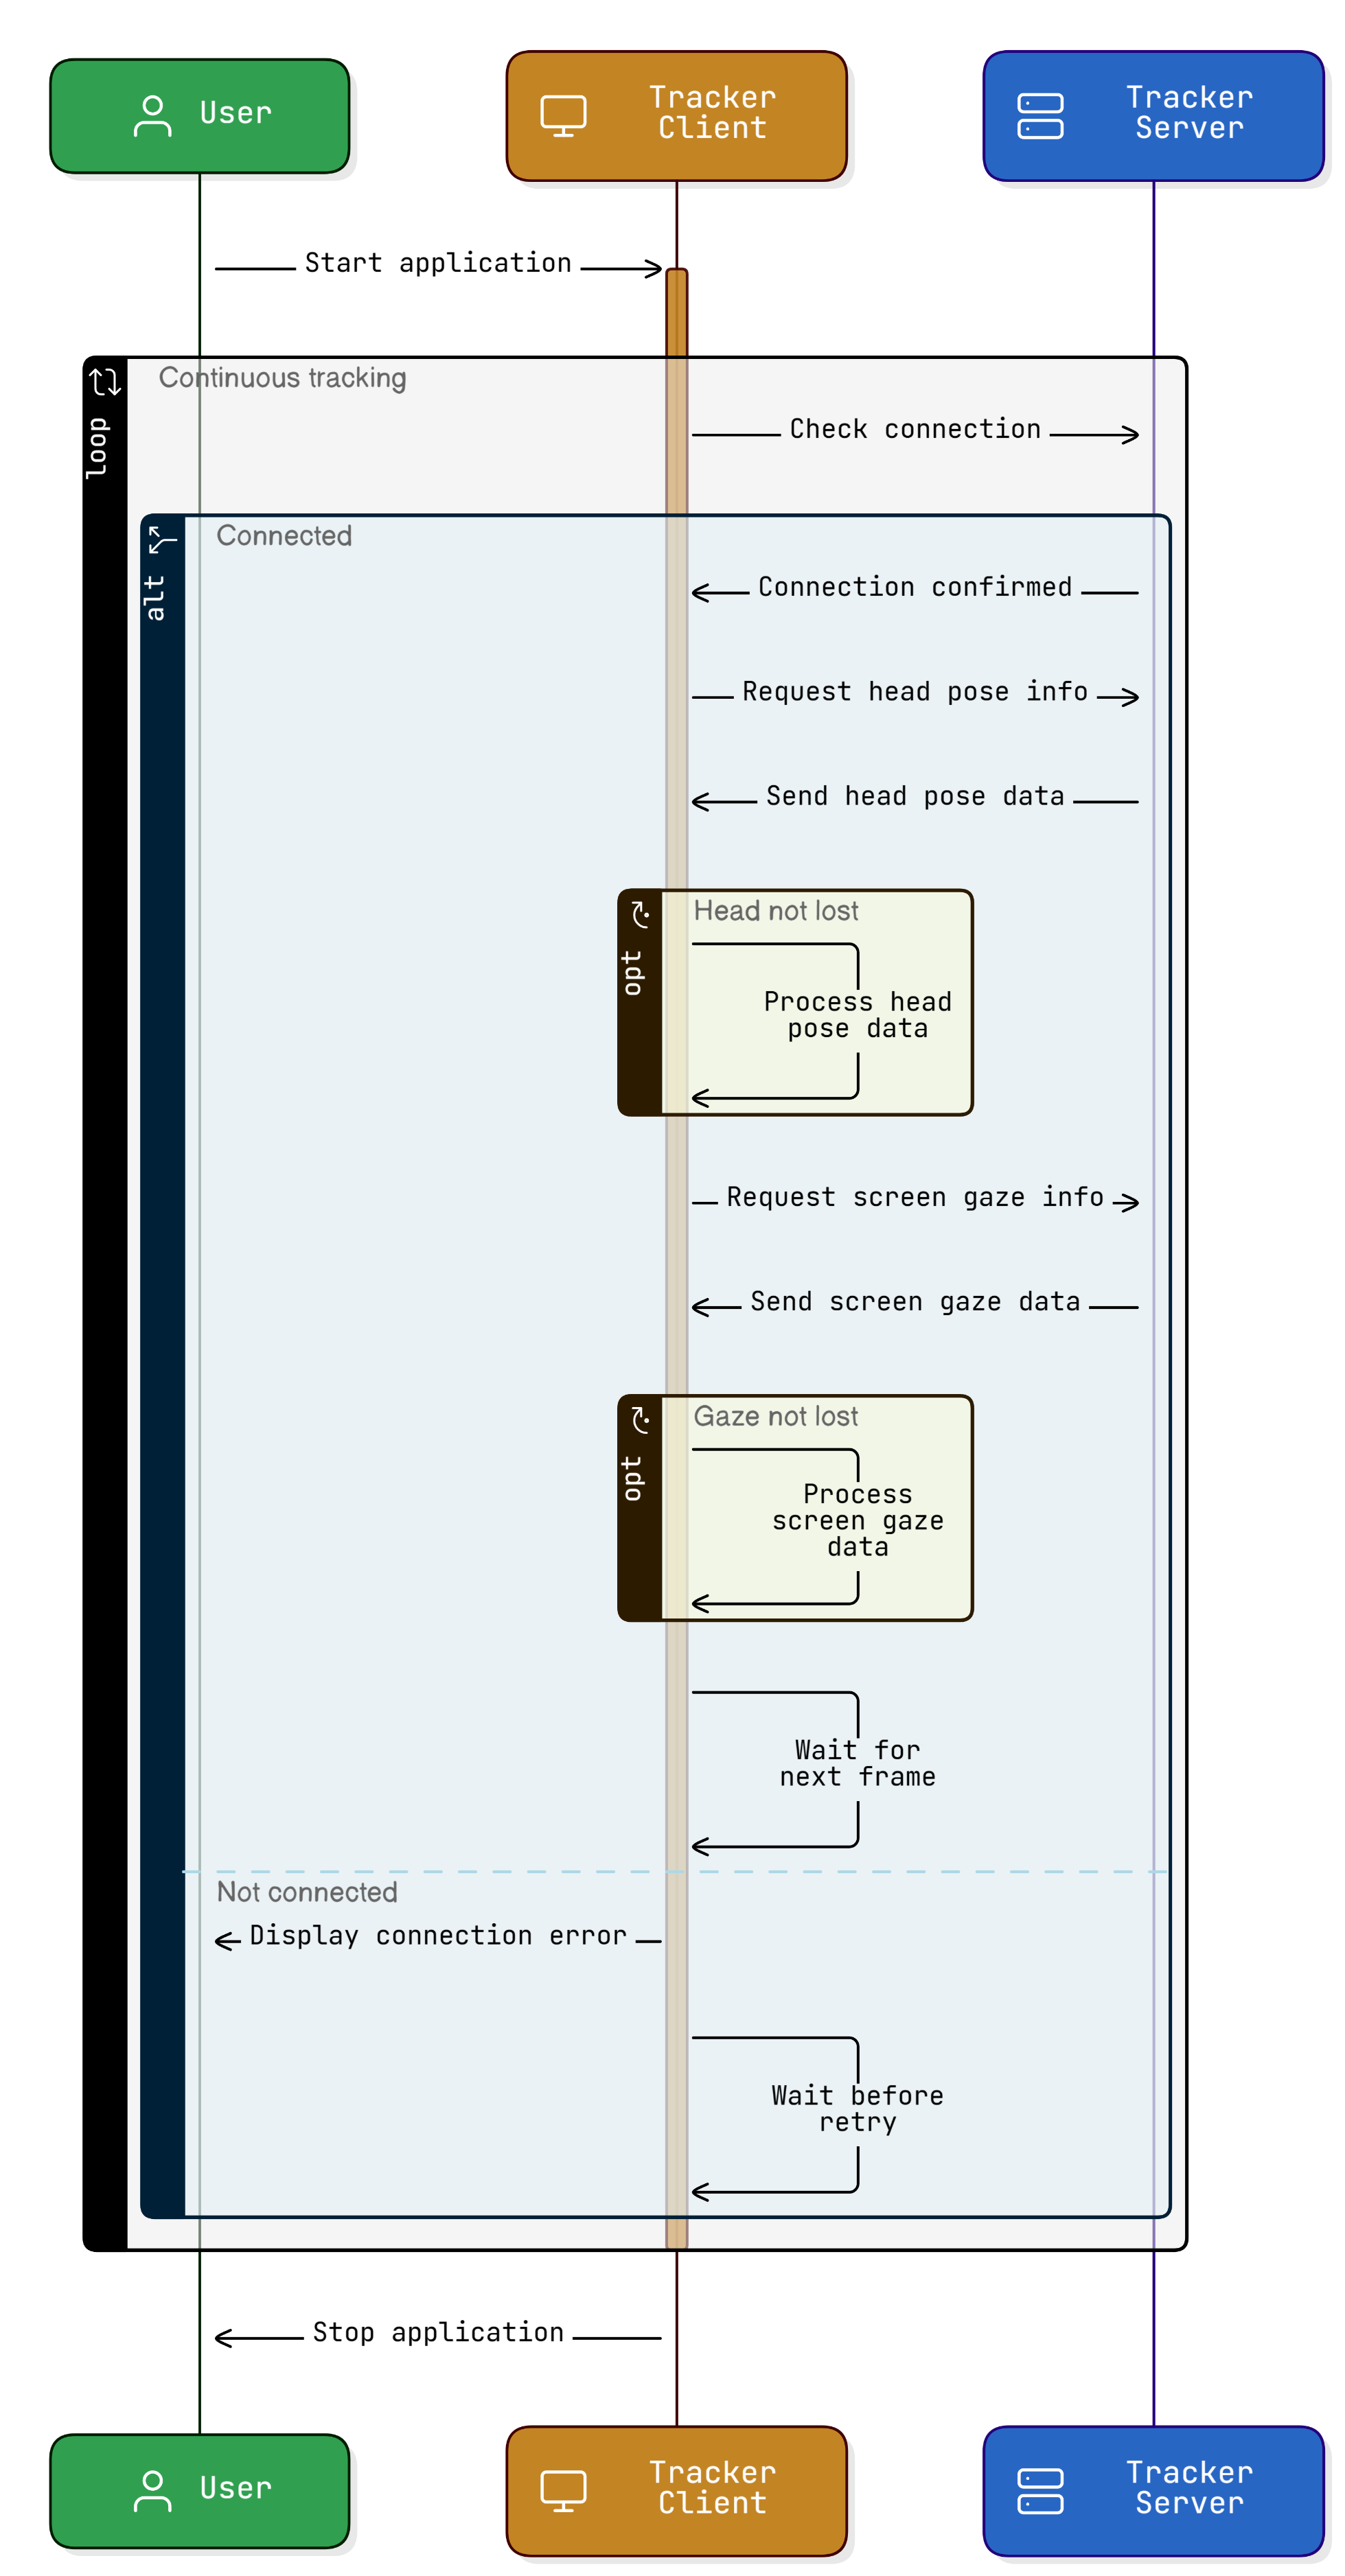
\includegraphics[scale=0.12]{code_structure_beam}
\caption{Visuelle Darstellung des Codes zur Beam SDK, Quelle: \cite{lit_code_beam_sdk}, \cite{lit_software_eraserio}} \label{fig:code_structure_beam}
\end{center}
\end{figure}


Die Funktionsweise der \acrshort{api} ist vereinfacht in Abbildung \ref{fig:code_structure_beam} zu erkennen. Der Tracker Server ist die Bezeichnung für den Eye Tracker selbst. Der Client ist das selbst geschriebene Programm, welches die Trackerdaten über die \acrshort{api} entgegennimmt. Die beiden Hauptinformation, welche vom Server an den Client übergeben werden sind die Daten zur Kopfposition (head pose data) und die Daten zur Blickposition (screen gaze data). Die Kopfposition gibt Auskunft über die Translation und Rotation des Kopfes der Testperson. Die Blickposition gibt Auskunft auf welchen Punkt auf dem Bildschirm die Testperson schaut. Diese beiden Systeme laufen unabhängig voneinander und dienen unterschiedlichen Einsatzzwecken. Das Kopftracking kann bspw. dazu verwendet werden, um die Kamera in einer Simulationswelt zu bewegen. Das könnte Sinn machen, wenn keine große Leinwand wie im Fahrsimulator vorhanden ist. Durch einen Blick nach links, könnte sich auch die Kamera im Fahrsimulator mit nach links bewegen. Für den Einsatzzweck im Fahrsimulator ist diese Funktion durch die große Leinwand allerdings nicht notwendig. Die Daten werden dennoch übermittelt, falls in Zukunft doch ein Anwendungsfall entstehen sollte. Die Gaze Daten sind das eigentlich Relevante. Diese geben eine Schätzung ab, auf welchen Punkt die Testperson auf der Leinwand schaut. Sofern eine Testperson vom Eye Tracker erkannt ist, werden in kontinuierlichen Abständen diese Daten vom Eye Tracker an den Client übermittelt. Zusätzlich dazu werden auch noch andere Daten wie bspw. die confidence übermittelt. Dabei handelt es sich um einen Wert, welcher mit jeder geschätzten Blickposition mit übermittelt wird. Dieser gibt an, wie sicher sich der Eye Tracker mit seiner Schätzung der aktuellen Blickposition ist. 

\subsection{Schnittstelle zu Carla}

Der Eye Tracker und Carla arbeiten größtenteils getrennt voneinander. Die visuelle Ausgabe des Eye Trackers erfolgt durch einen kleinen schwarzen Punkt, welcher die aktuell, geschätzte Blickposition auf der Leinwand anzeigt. Dieser schwarze Punkt befindet sich in einem transparenten Fenster, welches über die \acrshort{rgb}-Sensorausgabe gelegt ist. Es gibt auch einen sogenannten Textmanager. In diesem werden für den Nutzer unter anderem die grobe Blickrichtung in Textform angezeigt. Zum Beispiel "schaut nach oben links". Eine weitere Übergabe der Eye Tracker Daten erfolgt in eine Funktion, welche eine Krümmungs-Korrektur durchführt. Da die Leinwand im Fahrsimulator nicht gerade ist, sondern halbkreisförmig aufgebaut ist, muss diese Funktion den daraus resultierenden Fehler eliminieren. Das Problem der Krümmung und die dafür entwickelte Korrektur werden in einem späteren Abschnitt detailliert erläutert. 

Die einzige direkte Schnittstelle zwischen Carla und den Daten des Eye Trackers ist die Übergabe der Eye Tracker Daten an die Auswertung des Instance Segmentation Sensors. Diese Schnittstelle funktioniert so, wie in Abbildung \ref{fig:eye_tracker_data} dargestellt. Der Carla Server sendet die Sensordaten des Instance Segmentation Sensors an den Carla Client. Diese kommen bereits um den Faktor zehn kleiner an als die Sensordaten des \acrshort{rgb}-Sensors. Der Carla Client übergibt die Sensordaten an die Auswertung. Bei der Auswertung werden die Rohdaten des Eye Trackers, welche bereits eine Krümmungs-Korrektur erfahren haben, dann mit den Sensordaten des Instance Segmentation Sensors verarbeitet. Es erfolgt die Ausgabe, in welcher die Gruppenzugehörigkeit und die ID des Objektes enthalten sind. Diese Ausgabe wird dann im sogenannten "Text Manager" in Form von Text auf dem Bildschirm dargestellt. Die Darstellung des schwarzen Punktes bedient sich ebenfalls an den korrigierten Eye Tracker Daten, hat aber nichts mit dem Text Manager oder Carla zu tun. 

\begin{figure}[h!]
\begin{center}
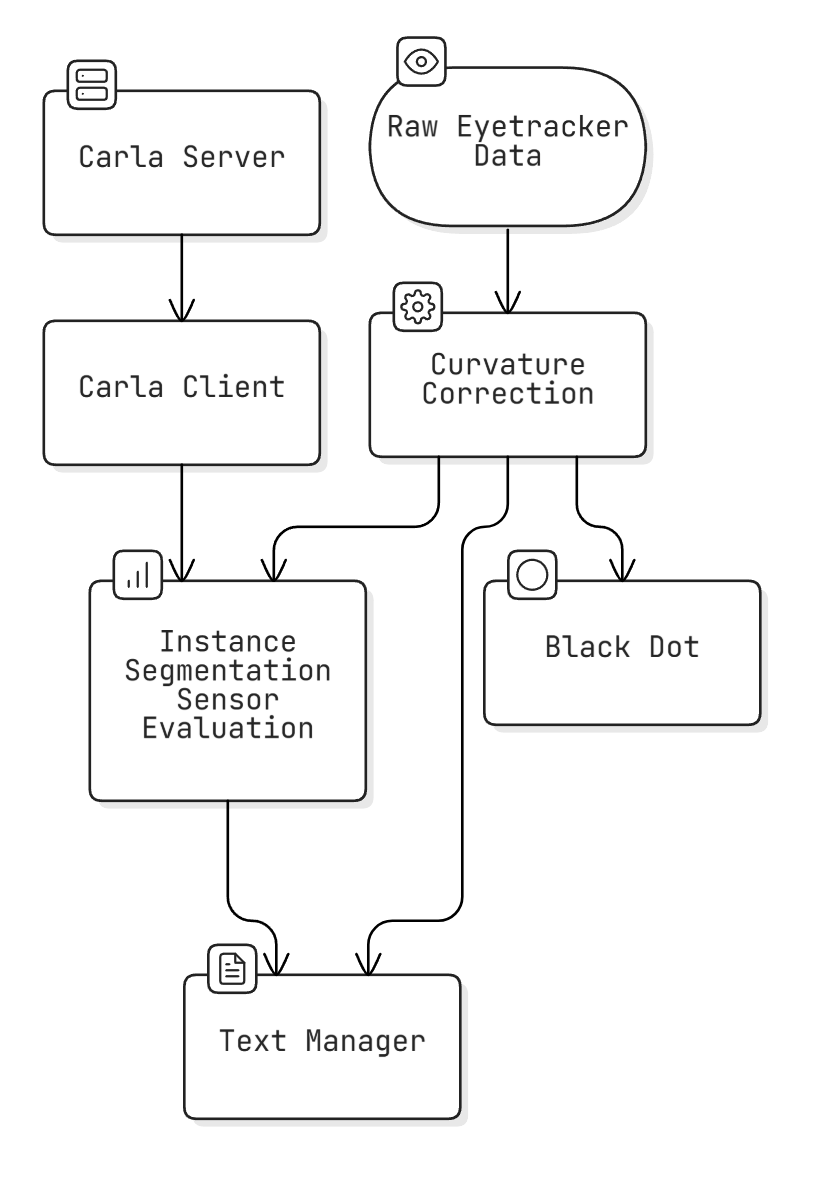
\includegraphics[scale=0.19]{eye_tracker_data}
\caption{Graphische Darstellung der Verarbeitung der Raw-Daten des Eye Trackers, Quelle: \cite{lit_website_carla_documentation}} \label{fig:eye_tracker_data}
\end{center}
\end{figure}



\section{Carla Umgebung}

\subsection{Aufbau Testszenario in Carla}

Um den Eye Tracker in Zusammenhang mit Carla testen zu können, muss eine Testumgebung in Carla angelegt werden. In Abbildung \ref{fig:code_structure_carla_1} sind die groben Schritte zur Erzeugung einer Testumgebung zu erkennen. Hier ist das Zusammenspiel zwischen dem Carla Server und dem Carla Client besonders hervorgehoben. Der Host-PC ist in diesem Fall der Computer, auf welchem der Fahrsimulator ausgeführt wird. Auf diesem ist Windows als Betriebssystem installiert. Im gesamten Zeitraum der Projektarbeit wird der Carla Server immer lokal auf diesem Computer laufen. Der Carla Server ist für die eigentliche Simulation sowie der Aktoren in ihr verantwortlich. Der Client läuft auf demselben Computer und kann Anfragen an den Server senden. Auf diese Weise kann der Client die Simulation aktiv beeinflussen oder Daten wie bspw. Positionsdaten oder Bilddaten vom Server anfragen. \cite{lit_website_carla_documentation}

Der Carla Server kann heruntergeladen werden und direkt als ausführbares Programm gestartet werden. Anders als der Carla Client, welcher selbst in Python geschrieben werden muss. Dafür kann dieser auch nach den eigenen Anforderungen individuell aufgesetzt werden. In der Dokumentation von Carla gibt es einige Beispiele wie ein Client aufgebaut werden kann, nach welchen sich der Client für diese Projektarbeit auch orientiert \cite{lit_code_api}. Zur Serververbindung nutzt er das Application Programming Interface (\acrshort{api}) des Carla Servers. Der Client wurde so geschrieben, dass er zuerst versucht, eine Verbindung zum Carla Server aufzubauen. Anschließend holt er sich wichtige Informationen über die simulierte Welt und mögliche \gls{Spawnpunkt}e für bspw. Fahrzeuge vom Server. Unter Actors werden in diesem Kontext unter anderem Fahrzeuge und Sensoren bezeichnet. Der Client fordert eine Liste aller in der aktuell simulierten Welt vorhandenen Fahrzeuge und Sensoren an und "zerstört" diese anschließend. Somit wird sichergestellt, dass keine Aktoren aus einer vorherigen Sitzung in die neue Sitzung mitgebracht werden. Nachdem die simulierte Welt wieder einen fest definierten Ausgangszustand angenommen hat, beginnt der Client damit, einen Mercedes Sprinter zu spawnen. Abbildung \ref{fig:code_structure_carla_2} stellt die Fortsetzung des Prozesses dar. Nachdem das Fahrzeug vom Server in der Welt erzeugt wurde, fordert der Client die Erzeugung von zwei Sensoren an. Beide Sensoren sollen an das erzeugte Fahrzeug geknüpft sein. Der erste Sensor soll den Rot-Grün-Blau (\acrshort{rgb})Farbraum erfassen. Der zweite Sensor soll die Instance Segmentation erfassen. Auf diese und die Verarbeitung der daraus resultierenden Daten wird weiter unten genauer eingegangen. 

\begin{figure}[h!]
\begin{center}
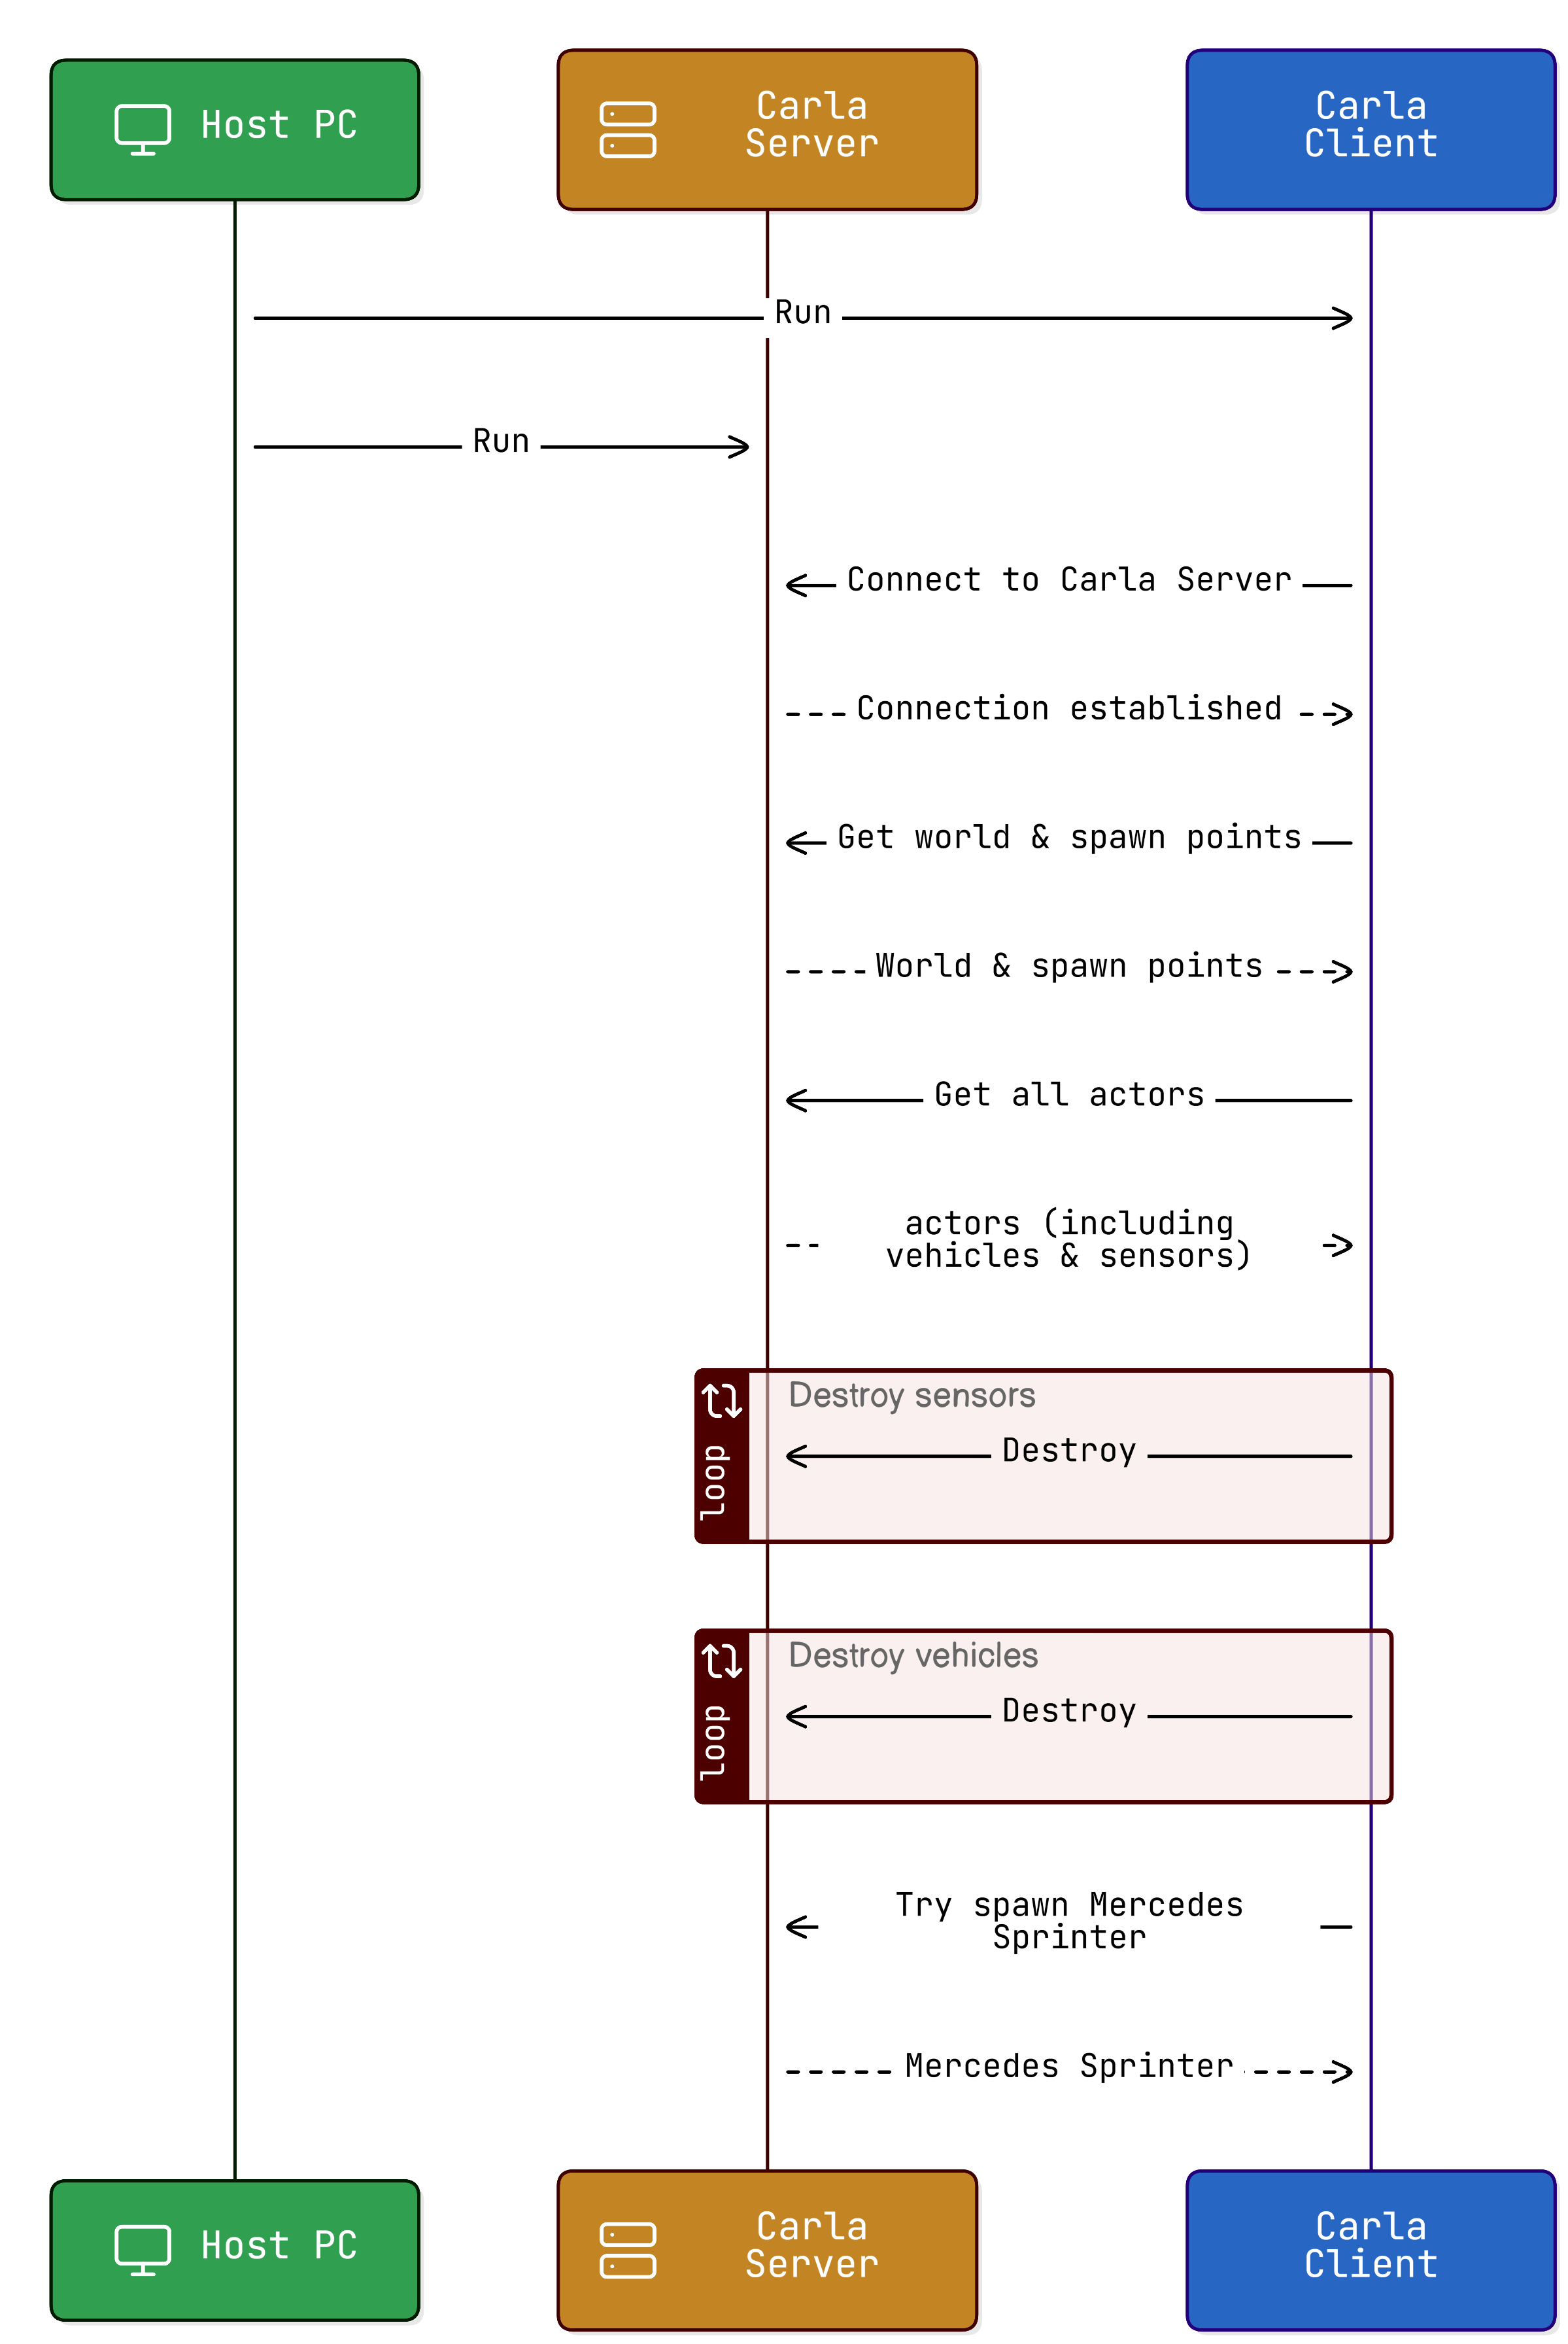
\includegraphics[scale=0.1]{code_structure_carla_1}
\caption{Visuelle Darstellung des Codes zur Carla Testumgebung Teil 1/2, Quelle: \cite{lit_software_eraserio},\cite{lit_website_carla_documentation}} \label{fig:code_structure_carla_1}
\end{center}
\end{figure}

\begin{figure}[h!]
\begin{center}
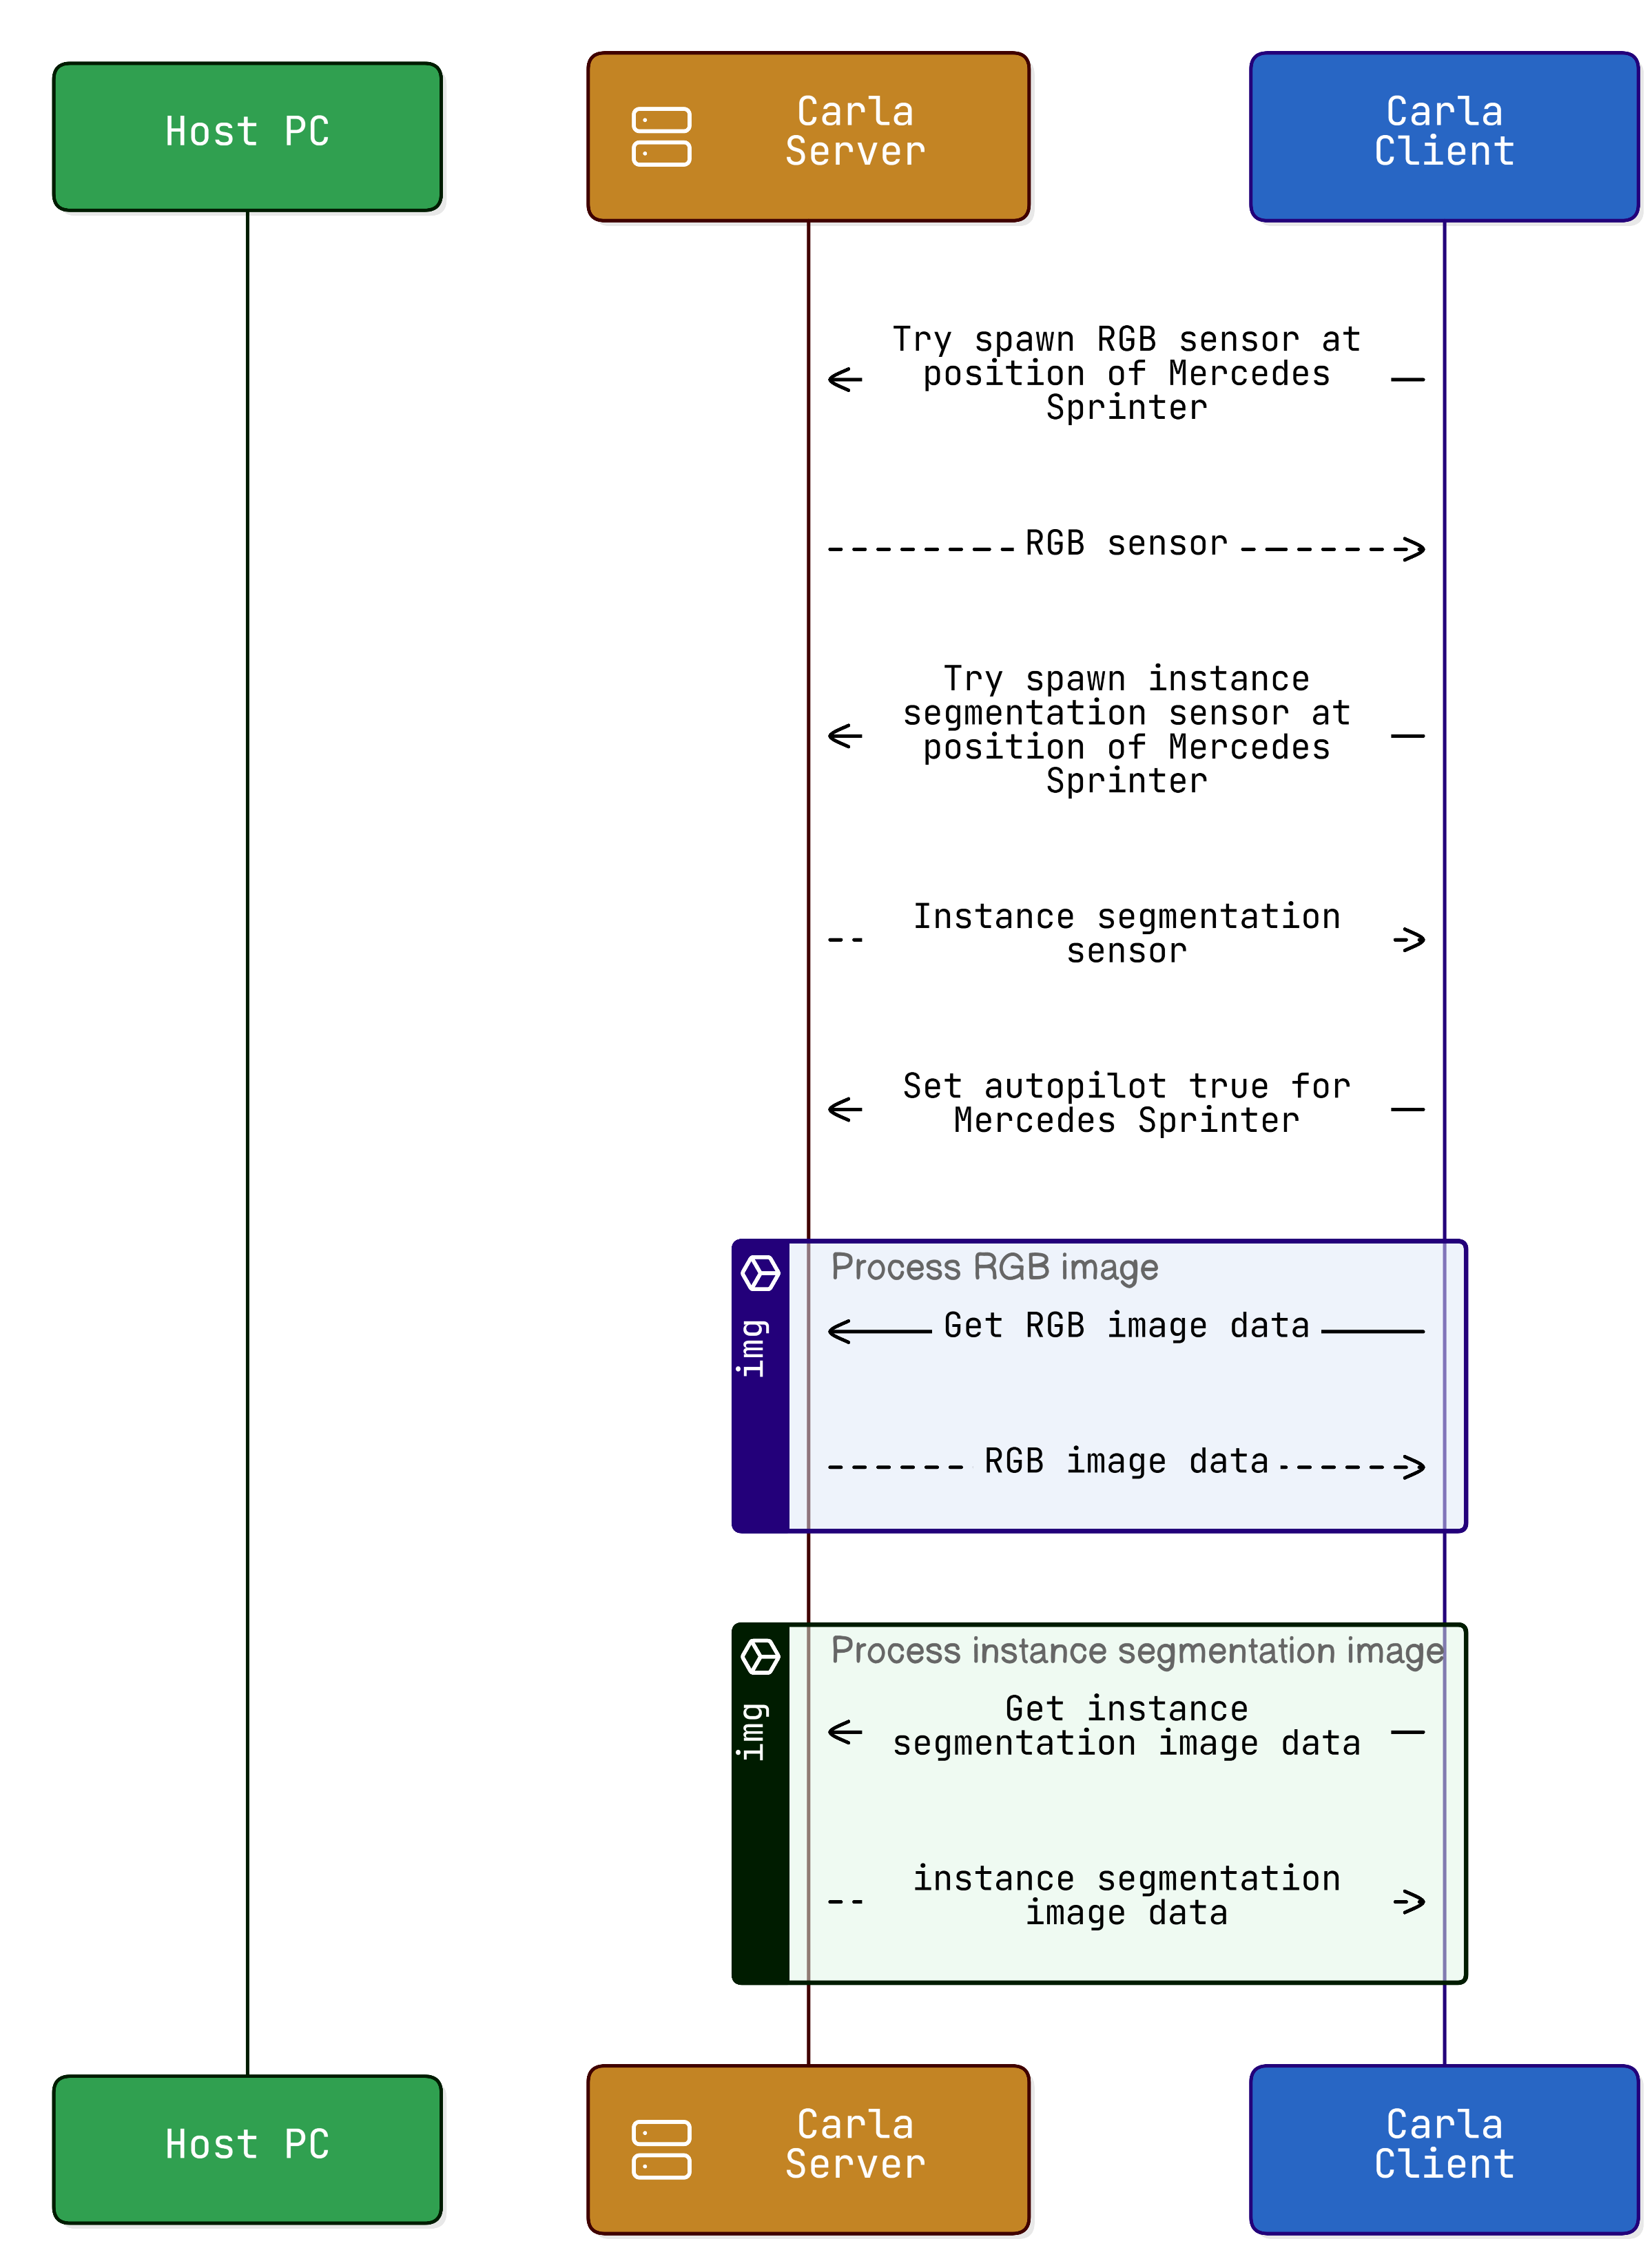
\includegraphics[scale=0.1]{code_structure_carla_2}
\caption{Visuelle Darstellung des Codes zur Carla Testumgebung Teil 2/2, Quelle: \cite{lit_software_eraserio},\cite{lit_website_carla_documentation}} \label{fig:code_structure_carla_2}
\end{center}
\end{figure}

\subsection{Sensor Auswertung}

\subsubsection{Verschiedene Sensortypen}
Der \acrshort{rgb}-Sensor liefert ein Bild an den Client, welches einer Kameraaufnahme gleicht. Durch die roten, grünen und blauen Farbanteile kann ein Bild erzeugt werden, welches für die Testperson im Fahrsimulator die simulierte Welt in Farbe darstellt. Die simulierte Welt kann durch diesen \acrshort{rgb}-Sensor wie durch eine Kameralinse betrachtet werden. Der Server berechnet die Welt in Zahlen und der Sensor ermöglicht es der Testperson im Fahrsimulator diese auf zahlen basierende Welt visuell wahrzunehmen. Die Objekte und die Farben der Welt werden so dargestellt, wie sie für den Menschen natürlich sind. Ein Baum hat die Form eines Baums und besitzt grüne Blätter und einen braunen Stamm. In Carla kann bei Bedarf auch ein Lidar-Sensor platziert werden. Dieser erzeugt ebenfalls ein Bild der simulierten Umgebung. Dieses würde den Baum dann aber als eine Art Punktwolke in einer schwarzen Umgebung darstellen. Ein Lidar-Sensor würde die Welt in einer anderen Art und Weise wahrnehmen, wodurch auch ein anderes Bild im Vergleich zu einem \acrshort{rgb}-Sensor entstehen würde. 

\subsubsection{Instance Segmentation Sensor}
Der Instance Segmentation Sensor ist in seiner Funktion etwas spezieller. Dieser kategorisiert die Objekte in der Welt in Gruppen ein und weißt ihnen IDs zu. Er färbt gewisse Objektgruppen nach ihrer jeweiligen Gruppenzugehörigkeit. Bspw. werden Straßen hellgrün und Gebäude dunkelblau gezeichnet. Zusätzlich besitzt jedes Objekt eine eindeutige Identifikationsnummer (\acrshort{id}). So hat jedes Fahrzeug in der simulierten Welt eine eindeutige, ihm zugewiesene \acrshort{id}. Damit sowohl die Gruppenzugehörigkeit, als auch die \acrshort{id} in die Bildinformation der Sensorausgabe übergeben werden können, gibt es zwei Codierungsmechanismen. Bei der Sensorausgabe handelt es sich wie beim \acrshort{rgb}-Sensor um eine Farbbildausgabe bestehend aus rot-, grün- und blau-Anteilen. Die Zugehörigkeit eines Objekts in eine bestimmte Gruppe wird durch den Rot-Anteil des Bildes an der Stelle des Objektes bestimmt. Die Tabelle \ref{tab:rot_tag} stellt die korrekte Zuweisung zwischen dem Rot-Wert und der jeweiligen Eingruppierung dar. Im Code wurde sich auf diese Zuweisung gestützt. Es muss berücksichtigt werden, dass bei unterschiedlichen Versionen von Carla eine unterschiedliche Zuweisung erfolgt \cite{lit_website_carla_documentation}. 


\begin{table}[h]
    \begin{center}
    {\small %
    \begin{tabular}{c l}
        \toprule
        \textbf{Rot-Wert} & \textbf{Gruppe} \\
        \midrule
        0  & Unlabeled \\
        1  & Roads \\
        2  & SideWalks \\
        3  & Building \\
        4  & Wall \\
        5  & Fence \\
        6  & Pole \\
        7  & TrafficLight \\
        8  & TrafficSign \\
        9  & Vegetation \\
        10 & Terrain \\
        11 & Sky \\
        12 & Pedestrian \\
        13 & Rider \\
        14 & Car \\
        15 & Truck \\
        16 & Bus \\
        17 & Train \\
        18 & Motorcycle \\
        19 & Bicycle \\
        20 & Static \\
        21 & Dynamic \\
        22 & Other \\
        23 & Water \\
        24 & RoadLine \\
        25 & Ground \\
        26 & Bridge \\
        27 & RailTrack \\
        28 & GuardRail \\
        \bottomrule
    \end{tabular}
    }%
    \end{center}
    \caption{Zuweisung Rot-Wert und Objektgruppe bei Carla Version 0.9.15, Quelle: \cite{lit_website_carla_documentation}}\label{tab:rot_tag}
    
\end{table}



Die \acrshort{id} wird in den grün- und blau-Anteil des Bildes codiert. Liegt bspw. ein grün-Anteil von 22 und ein blau-Anteil von 232 vor, dann lautet die \acrshort{id} des Objektes "22-232".

Der Client fordert die Sensorausgabe des Instance Segmentation Sensors in regelmäßigen Abständen vom Server an. Anschließend extrahiert er die \acrshort{rgb}-Werte und wertet diese nach den oben beschriebenen Zuordnungen aus. Die Auswertung erfolgt dabei immer genau an einem Pixel. Die Position des Pixels ist definiert durch die aktuelle Ausgabe der geschätzten Blickposition vom Eye Tracker. 

\subsubsection{Optimierung der Performance}
Der Rechenaufwand, den der Server leisten muss, um die Sensorausgabe zu generieren, ist nicht zu vernachlässigen. Bei der \acrshort{rgb}-Ausgabe sind nicht viele Abstriche möglich, da die Testperson ein Bild von hoher Auflösung für die große Leinwand im Fahrsimulator benötigt. Die Sensorausgabe des Instance Segmentation Sensors kann hingegen auch mit einer geringeren Auflösung generiert werden. Dadurch wird Rechenleistung gespart und da die Sensorausgabe nur im Hintergrund benötigt wird, macht es für die Testperson auch keinen bemerkbaren Unterschied. 

Damit das Zusammenspiel zwischen Eye Tracker und Sensor allerdings weiterhin funktioniert, müssen die Werte des Eye Trackers ebenfalls auf die herunterskalierte Sensorausgabe umgerechnet werden. In Abbildung \ref{fig:scale} ist diese Skalierung grafisch dargestellt. Durch den Faktor zehn werden aus den Originalbilddaten jeweils 10x10 Pixel auf ein einzelnes Pixel herunterskaliert. Alle Pixel innerhalb dieses 10x10 Rasters, wie bspw. das Pixel bei Position x=7 und y=4 werden dann auf ein Pixel bezogen. Dadurch wird offensichtlich die Genauigkeit verringert, da der Eye Tracker zwar Tracking Daten bezogen auf die Originalauflösung ausgibt, dann aber auf die herunterskalierte Instance Segmentation Sensorausgabe beziehen muss. Bei einer Reduzierung der Auflösung um Faktor zehn wurden allerdings keine bemerkbaren, negativen Einflüsse auf die Funktion des Eye Trackers festgestellt.



\begin{figure}[h]
    \begin{center}
    \begin{tikzpicture}[scale=0.6]
        % Großes Raster (Originale Auflösung)
        \draw[step=1cm, gray!50, very thin] (0,0) grid (10,10);
        \node at (5,-0.5) {Originale Auflösung (10x10)};
        
        % Kleines Raster (herunterskalierte Auflösung)
        
        \draw[step=1cm, black, thick] (12,0) grid (13,1);
        \node at (13,-0.5) {Skalierte Auflösung (1x1)};
        
        % Punkt in der großen Skala
        \fill[red] (7, 4) circle (3pt);
        \node[above] at (7, 4) {$(x,y) = (7,4)$};

        % Skalierter Punkt
        \fill[blue] (12.5,0.5) circle (3pt);
        \node[right] at (13,0.5) {$(x_{scaled}, y_{scaled}) = (1,1)$};

        % Pfeil zur Transformation
        \draw[->, thick] (7,4) -- (12.5,0.5);

    \end{tikzpicture}
    \caption{Herunterskalierung der Eye-Tracking-Daten um Faktor 10}\label{fig:scale}
    \end{center}
    
\end{figure}


\subsection{Darstellung der Daten in Carla}
Die Daten des Eye Trackers werden nicht direkt in Carla dargestellt, sondern in einem transparenten Windows Fenster, welches über die Carla Client Anwendung geschoben wird. Die Inhalte dieses transparenten Fensters können allerdings in Zukunft bei Bedarf in die Carla Anwendung selbst implementiert werden.

In Abbildung \ref{fig:carla_hud} ist die graphische Darstellung der Daten des Eye Trackers im transparenten Fenster zu erkennen. Das erste Anzeigeelement ist der lila gefärbte Kreis. Dieser zeigt die geschätzte Blickposition des Eye Trackers an. Bei den Werten handelt es sich um die Rohdaten, welche noch nicht durch unsere Korrekturfunktion bearbeitet wurden. Als zweites wird hier der rote Punkt angezeigt. In der Realität ist das der Mauszeiger. Zur besseren Sichtbarkeit wurde dieser durch einen roten Kreis hervorgehoben. Der Mauszeiger wurde dazu verwendet, um die Performance des Eye Trackers messbar zu machen. Die Testperson hat den Mauszeiger bewegt und auf diesen geschaut. Dadurch war der Wert der tatsächlichen Blickposition bekannt und konnte mit dem Wert für die geschätzte Blickposition verglichen werden. Während der normalen Verwendung des Eye Trackers spielt dieser aber keine Rolle. Als drittes Element wird der schwarze Punkt angezeigt. Dieser liefert genauso wie der lila farbene Kreis die geschätzte Blickposition auf der Leinwand. Allerdings werden für die Darstellung des schwarzen Punktes die von uns korrigierten Werte verwendet. Der schwarze Punkt ist dementsprechend der eigentlich geltende Wert. Das vierte Anzeigeelement ist die textbasierte Ausgabe. In dieser werden verschiedene Werte ausgegeben, welche gleich noch detaillierter beschrieben werden. Das kleine türkisfarbene Fenster oben links ist die Ausgabe des Instance Segmentation Sensors. Diese kann bei der Verwendung des Eye Trackers im Hintergrund laufen und muss nicht weiter beachtet werden.




\begin{figure}[h!]
\begin{center}
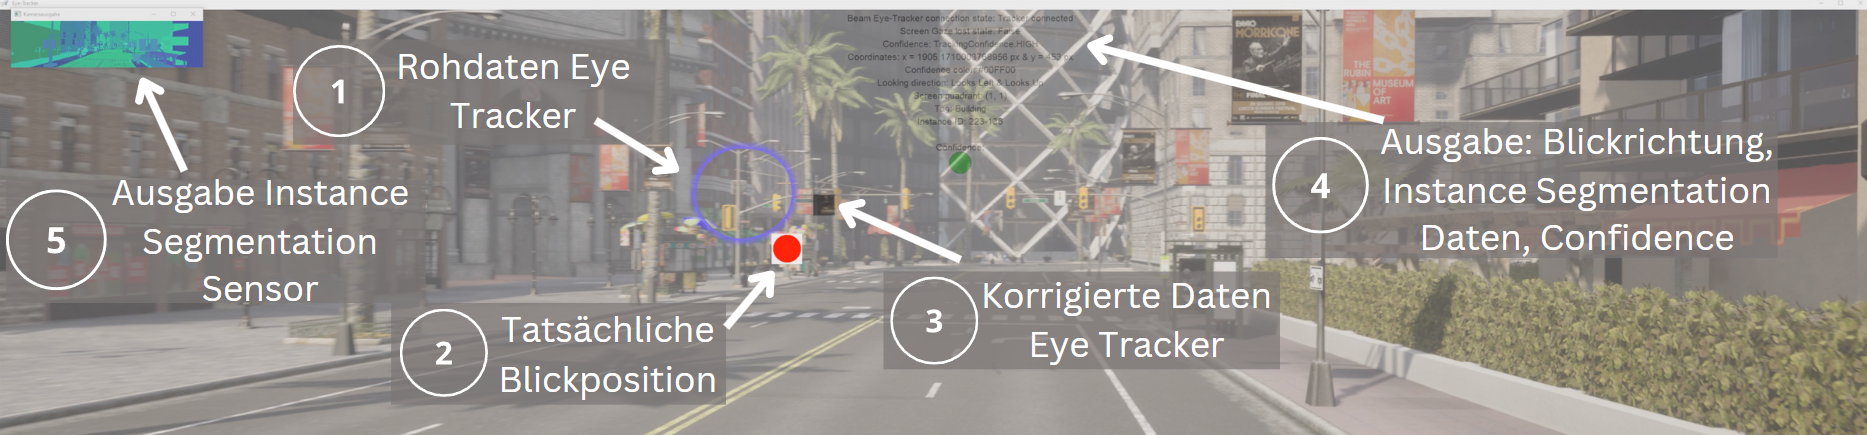
\includegraphics[scale=0.35]{carla_hud}
\caption{Darstellung der Daten in Carla, Quelle: \cite{lit_software_carla}, \cite{lit_software_canva}} \label{fig:carla_hud}
\end{center}
\end{figure}


In Abbildung \ref{fig:carla_hud_2} sind die textbasierten Daten aus Anzeigeelement vier in Abbildung \ref{fig:carla_hud} nochmals genauer dargestellt. Es werden Informationen über den Verbindungsstatus des Eye Trackers, die aktuell geschätzten Blickkoordinaten, die grobe Blickrichtung und die Instance Segmentation Auswertung gegeben. Die 'Looking Direction' gibt dabei die grobe Blickrichtung der Testperson an. Der 'Tag' ist die Einordnung des Objektes auf welches die Testperson schaut in eine Objektgruppe und die 'Instance ID' die eindeutige Identifikationsnummer für selbiges Objekt. Der grüne Punkt unten gibt die aktuelle Tracking Confidence des Eye Trackers nochmals in Form einer Ampel aus. Dadurch kann sofort erkannt werden, wenn der Eye Tracker die Testperson nicht mehr korrekt erfasst.  

\begin{figure}[h!]
\begin{center}
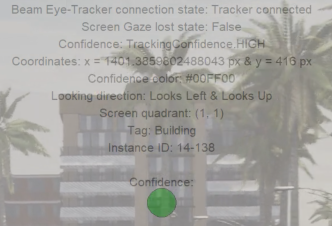
\includegraphics[scale=1]{carla_hud_2}
\caption{Darstellung textbasierten Daten in Carla, Quelle: \cite{lit_software_carla}, \cite{lit_software_canva}} \label{fig:carla_hud_2}
\end{center}
\end{figure}





\section{Korrektur gekrümmte Leinwand}
\subsection{Problemursache}
\subsubsection{Hauptproblem}
Die Leinwand des Fahrsimulators ist nicht flach sondern besitzt eine halbkreisförmige Form. Der Eye Tracker hat keine Einstellmöglichkeit, um eine gekrümmte Leinwand zu berücksichtigen. Dadurch entstehen starke Abweichungen zwischen der vom Eye Tracker geschätzten Blickposition und der realen Blickposition. Abbildung \ref{fig:kruemmungsproblem_1} visualisiert dieses Problem. 



\begin{figure}
\begin{center}
\begin{tikzpicture}
	%\draw [lightgray](0,0) grid (10,10);
	
	
	% Zeichnet die Flache Leinwand
	\draw[thick] (1,9) -- (9,9);
	
	% Zeichnet die linke und rechte Häfte des Halblreises der Leinwand
	\draw (2.45,6.45) arc (180:90:2.546479);
	\draw (7.55,6.45) arc (0:90:2.546479);
	
	% Zeichnet Kreis die Testperson darstellt 
	\fill[gray] (5, 6.5) circle [radius=0.2];
	
	% Zeichnet Pfeil 1 (zeigt direkten Blick nach vorne)
	\draw[thick][-stealth][red] (5,6.5) -- (5,9) node[midway, right, black] {$\mathbf{a.)}$};
	
	% Zeichnet Pfeil 2 (zeigt Blick nach links)
	\draw[thick][-stealth][red] (5,6.5) -- (1,9) node[midway, right, black] {$\mathbf{b.)}$};
	
	% Zeichnet Pfeil 3 (zeigt falsche Anzeige auf Bildschirm)
	\draw[thick][dashed][-stealth][blue] (5,6.5) -- (2.45,6.45) node[midway, below, black] {$\mathbf{c.)}$};
\end{tikzpicture}
\caption{Visualisierung der verzerrenden Wirkung einer gekrümmten Leinwand auf die Ergebnisse des Eye Trackers} \label{fig:kruemmungsproblem_1}
\end{center}
% Das Label wird gebraucht, um im Text auf diese Abbildung zu referenzieren
\end{figure}

In Abbildung \ref{fig:kruemmungsproblem_1} ist die gekrümmte Leinwand, sowie eine flache Leinwand zu erkennen. Aus Sicht des Eye Trackers existiert nur die flache Leinwand. Ein kleiner grauer Punkt visualisiert die Position der Testperson im Fahrsimulator. Pfeil a.) zeigt direkt von der Testpostion in einem Winkel von 0° auf die Mitte der Leinwand. Es ist zu erkennen, dass es in diesem Punkt keine Abweichung zwischen der flachen Leinwand und der gekrümmten Leinwand gibt. Aus diesem Grund ist zu erwarten, dass der Eye Tracker in diesem Punkt die genausten Ergebnisse liefert. 

Pfeil b.) zeigt ein zweites Szenario. Die Testperson schaut in diesem Fall nach links. Es ist zu erkennen, dass sie mit ihrem Blick die gekrümmte Leinwand auf der linken Seite etwas links von der Mitte trifft. Wenn der Blick der Testperson allerdings imaginär verlängert wird und dadurch auf die imaginäre, flache Leinwand trifft, wird die Abweichung erkennbar. Es ist zu erwarten, dass der Eye Tracker die Blickposition auf den linken Bildschirmrand schätzt, obwohl die reale Blickposition einen gewissen Abstand zum Bildschirmrand besitzt. In einem optimierten System würde der Eye Tracker die Blickposition, welche mit Pfeil b.) dargestellt ist, nur dann schätzen, wenn die Testperson auf den Punkt schaut, welcher mit Pfeil c.) dargestellt ist.


\subsubsection{Variabilität des Problems}

Es besteht kein gleichbleibender Zusammenhang zwischen der Blickposition auf der flachen Leinwand und der gekrümmten Leinwand. In Abbildung \ref{fig:kruemmungsproblem_2} sind zwei Beispiele zu erkennen. In Beispiel 1 wird der Blick auf die gekrümmte Leinwand mit dem Pfeil a.) dargestellt. Die Transformation auf die flache Leinwand wird mit Pfeil b.) visualisiert. Bei diesem Beispiel schaut die Testperson in einem Winkel $\alpha$ = 90° nach links. Zwischen dem Blick a.) und dem transformierten Blick b.) stellt sich ein Winkel ein. In Beispiel 2 wird nicht an den Bildschirmrand der gekrümmten Leinwand geschaut, sondern in die Mitte. Der Winkel $\beta$ = 45° stellt sich ein. Auch zwischen dem Blick c.) und dem transformierten Blick d.) stellt sich ein Winkel ein. Aus der Abbildung ist zu abzulesen, dass der Winkel zwischen b.) und a.) kleiner ist als der Winkel zwischen c.) und d.). Das zeigt, dass die Transformation zwischen der gekrümmten und der flachen Leinwand nicht konstant ist. Das Problem ist an den Rändern stärker ausgeprägt als in der Nähe der Mitte.

\begin{figure}
\begin{center}
\begin{tikzpicture}
%\draw [lightgray](0,0) grid (10,10);
	
	
% Zeichnet die Flache Leinwand
\draw[thick] (1,9.05) -- (9,9.05);
	
% Zeichnet die linke und rechte Häfte des Halblreises der Leinwand
\draw (2.45,6.5) arc (180:90:2.546479);
\draw (7.55,6.5) arc (0:90:2.546479);
	
% Zeichnet Kreis die Testperson darstellt 
\fill[gray] (5, 6.5) circle [radius=0.2];

% Zeichnet Pfeil 1 (zeigt direkten Blick nach vorne)
\draw[thick][black] (5,6.5) -- (5,9.05) node[midway, right, black] {$\mathbf{1.5 m}$} coordinate (direkt);
	
% Zeichnet Pfeil 2 (zeigt Blick nach links)
\draw[thick][-stealth][red] (5,6.5) -- (2.45, 6.5) node[midway, below, black] {$\mathbf{a.)}$} coordinate (blick);
	
%Ursprung zwischen den zwei Pfeilen 
\coordinate (O) at (5,6.45);

% Shorthandoff muss dazu geschrieben werden, weil es sonst durch das german Language Pack Probleme mit den Anführungszeichen kommt!
\shorthandoff{"}%
% Zeichnet einen Winkel zwischen den beiden Pfeilen 
\pic [draw, <->,
     angle radius=8mm, angle eccentricity=1.2,
     "$\alpha$"] {angle = direkt--O--blick};
\shorthandon{"}%
      
% Zeichnet Pfeil 3 (zeigt Transformation zwischen gekrümmter und flacher Leinwand)
\draw[thick][-stealth][blue] (2.45, 6.5) -- (1, 9.05) node[midway, right, black] {$\mathbf{b.)}$} coordinate;
	
	
	
% Zeichnet Pfeil 3 (zeigt Blick nach links weiter in Mitte)
\draw[thick][-stealth][red] (5,6.55) -- (3.22, 8.3) node[midway, left, black] {$\mathbf{c.)}$} coordinate (blick2);
	
% Zeichnet Pfeil 4 (Transformatio von c.) zu flacher Leinwand)
\draw[thick][-stealth][blue] (3.22, 8.3) -- (3, 9.05) node[midway, left, black] {$\mathbf{d.)}$} coordinate;

\shorthandoff{"}%
% Zeichnet einen zweiten Winkel zwischen den beiden weiteren Pfeilen 
\pic [draw, <->,
     angle radius=12mm, angle eccentricity=1.2,
     "$\beta$"] {angle = direkt--O--blick2};
\shorthandon{"}%
      
% Zeichnet Pfeil 3 (zeigt Transformation zwischen gekrümmter und flacher Leinwand)
\draw[thick][-stealth][blue] (2.45, 6.5) -- (1, 9.05) node[midway, right, black] {$\mathbf{b.)}$} coordinate;

\end{tikzpicture}
\caption{Visualisierung der nichtlinearen Transformation} \label{fig:kruemmungsproblem_2}
\end{center}
\end{figure}



\subsubsection{Problem der Sitzposition}

In den Abbildungen \ref{fig:kruemmungsproblem_1} und \ref{fig:kruemmungsproblem_2} wurde die Sitzposition der Testperson im Fahrsimulator immer im Mittelpunkt der gekrümmten Leinwand angekommen. In der Realität sitzt die Testperson nicht in der Mitte des Halbkreises, sondern näher in Richtung Leinwand. Ein Mensch hat ein Sichtfeld von ca. 200° \cite{lit_website_doccheck_fov}. Würde die Testperson in der Mitte des Halbkreises sitzen, dann würde die Leinwand 180° des Sichtfeldes umfassen. Da die Testperson aber näher an der Leinwand sitzt und somit nicht mehr in der Mitte des Halbkreises, befinden sich die Ränder der Leinwand weiter hinten und das Sichtfeld wird noch weiter ausgereizt. Kopfbewegungen im Eye Tracker sind nicht optimal. Da die Ränder der Leinwand nur durch eine kleine Kopfbewegung in das Sichtfeld rutschen, resultiert daraus eine verringerte Genauigkeit des Eye Trackers in der Nähe der Bildschirmränder.

Eine weitere Abweichung von den Annahmen weiter oben ist die um links verschobene Sitzposition der Testperson im Fahrsimulator. Bisher wurde angenommen, dass die Testperson direkt gegenüber der Mitte der Leinwand sitzt. In der Realität ist sie durch das nachgebaute Fahrzeugcockpit leicht nach links versetzt. Dadurch verhält sich die Transformation von flacher auf gekrümmte Leinwand links anders als rechts. Abbildung \ref{fig:kruemmungsproblem_3} visualisiert diese Einflüsse. 


\begin{figure}
\begin{center}
\begin{tikzpicture}
%\draw [lightgray](0,0) grid (10,10);
	
	
	% Zeichnet die Flache Leinwand
	\draw[thick] (1,9.05) -- (9,9.05);
	
	% Zeichnet die linke und rechte Häfte des Halblreises der Leinwand
	\draw (2.45,6.5) arc (180:90:2.546479);
	\draw (7.55,6.5) arc (0:90:2.546479);
	
	% Zeichnet Kreis die Testperson darstellt 
	\fill[gray] (4, 7) circle [radius=0.2];
	
	% Zeichnet Pfeil 1 (zeigt direkten Blick nach vorne)
	\draw[-stealth][thick][black] (4,7) -- (5,9.05) node[midway, right, black] {$\mathbf{}$} coordinate (direkt);
	
	% Zeichnet Pfeil 2 a.)(zeigt Blick nach links)
	\draw[thick][-stealth][red] (4,7) -- (2.45, 6.5) node[midway, below, black] {$\mathbf{a.)}$} coordinate (blick);
	
%Ursprung zwischen den zwei Pfeilen 
\coordinate (O) at (4,7);


      
      
	% Zeichnet Pfeil 3 b.) (zeigt Transformation zwischen gekrümmter und flacher Leinwand)
	\draw[thick][-stealth][blue] (2.45, 6.5) -- (1, 9.05) node[midway, right, black] {$\mathbf{b.)}$} coordinate (blick_transform);
	
	
	
% Zeichnet Pfeil 4 c.)(zeigt Blick nach links weiter in Mitte)
	\draw[thick][-stealth][red] (4,7) -- (3.22, 8.3) node[midway, left, black] {$\mathbf{c.)}$} coordinate (blick2);
	
% Zeichnet Pfeil 5 d.) (Transformatio von c.) zu flacher Leinwand)
	\draw[thick][-stealth][blue] (3.22, 8.3) -- (3, 9.05) node[midway, left, black] {$\mathbf{d.)}$} coordinate (blick2_transform);
	
	
% Zeichnet Pfeil 6 e.)(zeigt Blick nach rechts)
	\draw[thick][-stealth][red] (4,7) -- (7.55, 6.5) node[midway, below, black] {$\mathbf{e.)}$} coordinate (blick3);
	
% Zeichnet Pfeil 7 f.) (Transformatio von e.) zu flacher Leinwand)
	\draw[thick][-stealth][blue] (7.55, 6.5) -- (9, 9.05) node[midway, left, black] {$\mathbf{f.)}$} coordinate (blick3_transform);
	
\end{tikzpicture}
\caption{Visualisierung der Verschiebung der Sitzposition der Testperson} \label{fig:kruemmungsproblem_3}
\end{center}
\end{figure}

Es ist zu erkennen, dass in diesem Szenario vor allem zwischen der Blickrichtung c.) und der Transformation d.) kaum Fehler besteht. Durch die Sitzposition weiter links wird dort eine geringere Abweichung zwischen gekrümmter und flacher Leinwand bestehen. Experimente am Fahrsimulator haben diese Annahme bestätigt. Besonders in der Mitte der linken Seite hat der Eye Tracker gut geschätzt. Weiter links und sehr weit rechts wurde die Genauigkeit ohne eine Transformation auf die gekrümmte Leinwand wesentlich schlechter. 



\subsection{Lösungsansatz}

Wie im Abschnitt davor bereits beschrieben, muss eine Transformation zwischen den beiden Leinwänden durchgeführt werden. Die Richtung der Transformation wird dabei durch die Datengrundlage bestimmt. Die Daten stammen vom Eye Tracker und dieser geht von einer flachen Leinwand aus. Dementsprechend muss die Transformation von der flachen Leinwand auf die gekrümmte Leinwand stattfinden. 
Die Sitzposition und der Blinkwinkel bestimmen, wie die Transformation durchzuführen ist. 

Bei der Transformation ist nur die Horizontale von Relevanz. Vertikale Pixel müssen nicht transformiert werden, weil die Leinwand zwar horizontal gekrümmt ist aber nicht vertikal. Es besteht kein vertikaler Fehler zwischen der flachen und der gekrümmten Leinwand. Zu Zwecken der Nachvollziehbarkeit werden zu Beginn zwei einzelne Pixel betrachtet, welche von der flachen Leinwand auf die gekrümmte Leinwand projiziert werden sollen. Beide Pixel sollen sich auf der linken Hälfte der flachen Leinwand befinden. Abbildung \ref{fig:kruemmungsproblem_4} stellt den resultierenden Fehler bei gegebener Sitzposition und Blickrichtung dar. 



\begin{figure}
\begin{center}
\begin{tikzpicture}
	%\draw [lightgray](0,0) grid (10,10);
	
	
	% Zeichnet die Flache Leinwand
	\draw[thick] (1,9.05) -- (9,9.05);
	
	% Zeichnet die linke und rechte Häfte des Halblreises der Leinwand
	\draw (2.45,6.5) arc (180:90:2.546479);
	\draw (7.55,6.5) arc (0:90:2.546479);
	
	% Zeichnet Kreis die Testperson darstellt 
	\fill[gray] (4, 7) circle [radius=0.2];
	
	% Zeichnet Pfeil 1 (zeigt direkten Blick nach vorne)
	\draw[-stealth][thick][black] (4,7) -- (5,9.05) node[midway, right, black] {$\mathbf{a.)}$} coordinate (direkt);
	
%Ursprung zwischen den zwei Pfeilen 
\coordinate (O) at (4,7);
	
% Zeichnet Pfeil 4 c.)(zeigt Blick nach links weiter in Mitte)
	\draw[thick][-stealth][red] (4,7) -- (3.22, 8.3) node[right,yshift=-4pt, black] {$\mathbf{d.)}$} coordinate (blick2);
	
% Zeichnet Pfeil 5 d.) (Transformatio von c.) zu flacher Leinwand)
	\draw[thick][-stealth][blue] (3.22, 8.3) -- (3, 9.05) node[midway, right, black] {$\mathbf{c.)}$} coordinate (blick2_transform);
	
	
	% Zeichnet Pfeil 3 d.) (Zeigt Pfeil ohne korrigierende Transformation)
	\draw[thick][-stealth][green] (3.95,7) -- (2.7, 9.05) node[midway, left, yshift=12pt,xshift=-6pt, black] {$\mathbf{b.)}$} coordinate (blick_transform);
	
\shorthandoff{"}%	
\pic [draw, <->,
      angle radius=8mm, angle eccentricity=1.2,
      "$\alpha$", right] {angle = direkt--O--blick2};
\shorthandon{"}%

\shorthandoff{"}%
% Zeichnet den Fehler ein 
\draw [thick](2.7,9.1) -- (3,9.1)
node[midway,above , black] {$\mathbf{\Delta F}$};
\shorthandon{"}%
	
\end{tikzpicture}
\caption{Graphische Darstellung des Lösungsansatzes für die Transformation} \label{fig:kruemmungsproblem_4}
\end{center}
% Lösungsansatz zur Transformation
\end{figure}

In Abbildung \ref{fig:kruemmungsproblem_4} ist der Vektor von der Sitzposition zur Mitte der gekrümmten Leinwand durch a.) gegeben. Die Testperson schaut bezogen auf die gekrümmte Leinwand in Richtung Pfeil d.). Der Eye Tracker würde jetzt allerdings den Punkt auf welchen Pfeil b.) zeigt erkennen. Dieser würde wiederum mit einem anderen Punkt auf dem Halbkreis korrespondieren. Welcher in der Abbildung nicht dargestellt wird, weil es sonst zu unübersichtlich wird. Wichtig ist, dass die Ausgabe des Eye Trackers so transformiert wird, dass er anstatt den Punkt auf welchen Pfeil b.) zeigt, den Punkt, auf welchen Pfeil c.) zeigt, ausgibt. Es muss also eine Transformation um den Fehler $\Delta$ F stattfinden.


Die Berechnung von $\Delta$ F ist ein mathematisches Problem. Durch die nach links verschobene Sitzposition und die fehlenden Längenangaben der einzelnen Pfeile ist die Berechnung recht komplex. Ein alternativer Ansatz wäre eine Funktion, welche grob eine Transformation durchführt und vor Ort feinjustiert wird. In Abbildung \ref{fig:kruemmungsproblem_5} ist zu erkennen, dass bei einem Blick in die Mitte der linken Hälfte der gekrümmten Leinwand, eine leichte Korrektur nach rechts notwendig ist. Schaut man auf den Pfeil c.) aus Abbildung \ref{fig:kruemmungsproblem_5} wird klar, dass auf der rechten Seite der Halbkugel eine Korrektur nach links notwendig ist und diese stärker ausfallen muss, als auf der linken Seite. Aus den vorherigen Abbildungen ist zudem herauszulesen, dass das Problem umso stärker wird, je näher sich der Blick den Rändern der Leinwand annähert. Dabei ist es egal, ob linke Hälfte oder rechte Hälfte. 
Allerdings befindet sich der Punkt, welcher keine Korrektur benötigt, nach wie vor in der Mitte der Leinwand, unabhängig von der Sitzposition der Testperson.

\begin{figure}
\begin{center}
\begin{tikzpicture}
	%\draw [lightgray](0,0) grid (10,10);
	
	
	% Zeichnet die Flache Leinwand
	\draw[thick] (1,9.05) -- (9,9.05);
	
	% Zeichnet die linke und rechte Häfte des Halblreises der Leinwand
	\draw (2.45,6.5) arc (180:90:2.546479);
	\draw (7.55,6.5) arc (0:90:2.546479);
	
	% Zeichnet Kreis die Testperson darstellt 
	\fill[gray] (4, 7) circle [radius=0.2];
	
	% Zeichnet Pfeil 1 (zeigt direkten Blick nach vorne)
	\draw[-stealth][thick][black] (4,7) -- (5,9.05) node[midway, right, black] {$\mathbf{}$} coordinate (direkt);
	
%Ursprung zwischen den zwei Pfeilen 
\coordinate (O) at (4,7);


	
% Zeichnet Pfeil 4 c.)(zeigt Blick nach links weiter in Mitte)
	\draw[thick][-stealth][red] (4,7) -- (3.22, 8.3) node[midway, left, black] {$\mathbf{a.)}$} coordinate (blick2);
	
% Zeichnet Pfeil 5 d.) (Transformatio von c.) zu flacher Leinwand)
	\draw[thick][-stealth][blue] (3.22, 8.3) -- (3, 9.05) node[midway, left, black] {$\mathbf{b.)}$} coordinate (blick2_transform);


	
% Zeichnet Pfeil 4 c.)(zeigt Blick nach links weiter in Mitte)
	\draw[thick][-stealth][red] (4,7) -- (6.82, 8.3) node[midway, left, black] {$\mathbf{c.)}$} coordinate (blick2);
	
% Zeichnet Pfeil 5 d.) (Transformatio von c.) zu flacher Leinwand)
	\draw[thick][-stealth][blue] (6.82, 8.3) -- (7, 9.05) node[midway, right, black] {$\mathbf{d.)}$} coordinate (blick2_transform);
	
	
\end{tikzpicture}
\caption{Bestimmung der notwendigen Korrektur auf beiden Halbseiten des Halbkreises} \label{fig:kruemmungsproblem_5}
\end{center}
% Lösungsansatz zur Transformation
\end{figure}

\subsubsection{Mathematischer Ansatz e-Funktion}

Um die Transformation durchzuführen wird folgende selbst entwickelte Formel verwendet:

\begin{equation} 
	k=e^{c*(w-p)} \label{eq:1}
\end{equation}

Dabei ist: 
\begin{center}
	k - Korrektur-Wert\par
	c - Korrektur-Koeffizient (zum Einstellen der Korrektur)\par
	w - Bildschirmbreite in Pixel geteilt durch zwei \par
	p - Zu korrigierender Pixel \par
\end{center}

Des weiteren gelten folgende Formeln: 

\begin{equation} 
	p_{k,l}=p+k \label{eq:2}
\end{equation}

Dabei ist: 
\begin{center}
	$p_{k,l}$ - Korrigierter Pixel links\par
	p - Zu korrigierender Pixel \par
	k - Korrektur-Wert\par
\end{center}

Die Gleichung ref{eq:2} wird nur auf der linken Bildschirmhälfte angewandt. Der Korrektur-Wert k bestimmt dabei die Pixel, um welche man die Position des Eye-Trackers verschieben muss. Da es sich um die linke Bildschirmhälfte handelt, muss nach rechts korrigiert werden. Auf den vom Eye-Tracker bestimmten Pixel muss also der Korrektur-Wert aufsummiert werden. Wir müssen sozusagen vom linken Bildschirmrand weg eine Korrektur in Richtung Bildschirmmitte durchführen. 

\begin{figure}[h!]
\begin{center}
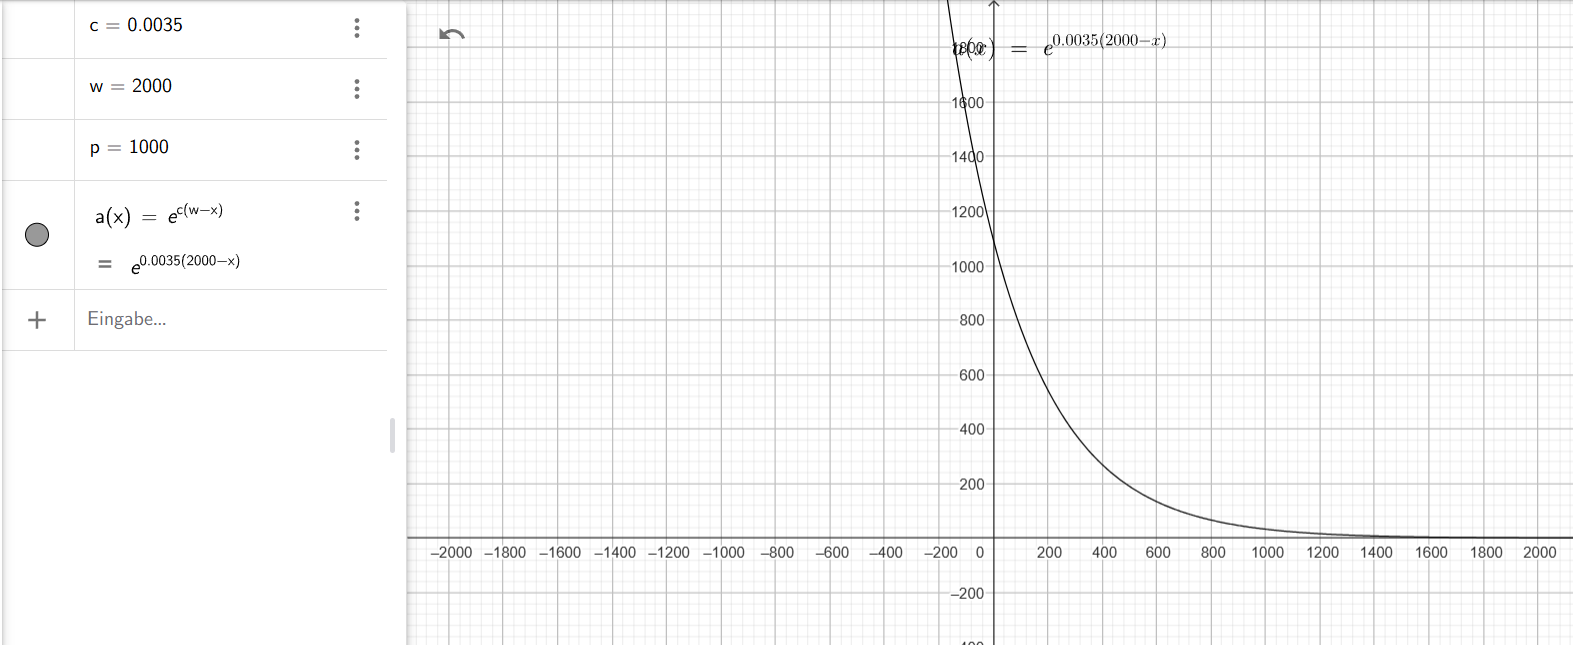
\includegraphics[scale=0.4]{Geogebra_links}
\caption{Sinnvolle Werte für den Korrekturfaktor linke Bildschirmhälfte} \label{fig:imag6}
\end{center}
\end{figure}

In der Abbildung ist zu erkennen für welchen Korrektur-Koeffizienten bei einer Leinwand mit 4000 Pixeln Breite sinnvolle Werte zu erzielen sind. Bei 4000 Pixeln Gesamtbreite, also 2000 Pixeln auf der linken Bildschirmhälfte wäre c=0.0035 ein realistischer Wert. 


\begin{figure}[h!]
\begin{center}
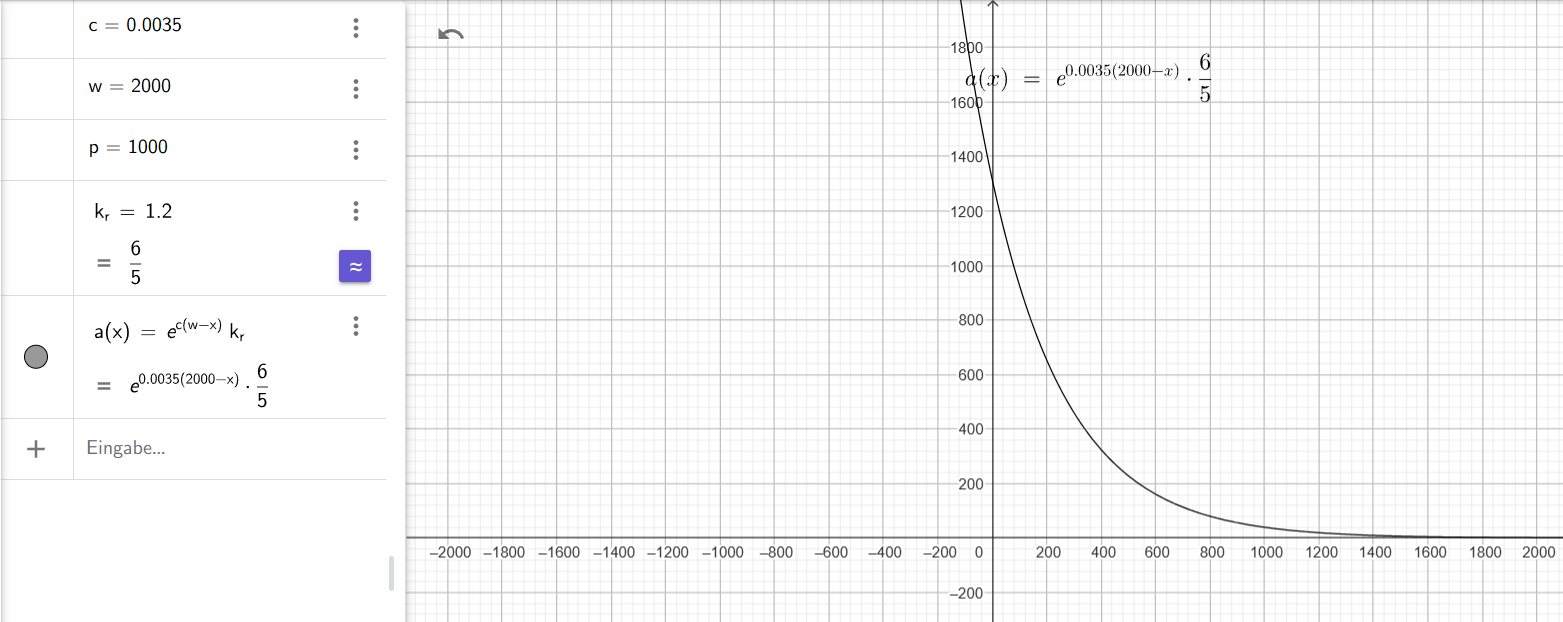
\includegraphics[scale=0.4]{Geogebra_rechts}
\caption{Sinnvolle Werte für den Korrekturfaktor rechte Bildschirmhälfte} \label{fig:imag7}
\end{center}
\end{figure}

In der Abbildung sind sinnvolle Werte für die rechte Bildschirmhälfte zu erkennen. Beim Korrekturfaktor c ändert sich nichts. Der zusätzlich hinzugekommene Korrekturfaktor $p_{k,r}$ wurde in diesem Beispiel mit 1.2 ausgewählt. 

Die Feinabstimmung muss experimentell am Fahrsimulator durchgeführt werden.

Der Korrekturfaktor muss für die rechte Bildschirmhälfte leicht verändert gerechnet werden. Angenommen die halbe Bildschirmbreite w beträgt 2000 Pixel. Die größte Korrektur findet am Rand statt also bei 2*w=4000 Pixel. Dort ist es dann: 2000-(4000-4000)=2000. In der Mitte soll keine Korrektur stattfinden. Dort ist es dann: 2000-(4000-2000)=0. 

\begin{equation} \label{eq:3}
	k=e^{c*(w-(2*w-p)}
\end{equation}


\begin{equation} \label{eq:4}
	p_{k,r}=p-k*k_r
\end{equation}

Dabei ist: 
\begin{center}
	$p_{k,r}$ - Korrigierter Pixel links\par
	p - Zu korrigierender Pixel \par
	k - Korrektur-Wert\par
	$k_r$ - Zusätzlicher Korrektur-Koeffizient für rechte Seite \par
\end{center}

\noindent Die Gleichung ref{eq:3} wird nur auf der rechten Bildschirmhälfte angewandt. Die bei der rechten Seite wird anders als bei der linken Seite nach links und nicht nach rechts korrigiert. Aus diesem Grund wird in der Formel mit einem negativen Vorzeichen gerechnet. Zusätzlich gibt es einen weiteren Koeffizient $k_r$. Dieser stellt sicher, dass die Korrektur auf der rechten Bildschirmseite leicht stärker ausfällt, da die durch die links ausgerichtete Sitzposition der Testperson notwendig ist. 

Der mathematische Ansatz wurde im Fahrsimulator getestet und es konnten zwar Verbesserungen festgestellt werden, allerdings gab es noch einige Probleme und Optimierungsbedarf. Die Korrektur in der Mitte des Bildschirms ist wesentlich zu schwach. Auch im mittleren Bereich ist sie zu schwach. Zudem sind in Richtung Ränder große Einbußen des Sichtfeldes zu bemängeln. Eine detaillierte Auswertung der Ergebnisse wird hier übersprungen, da schon durch bloßes Hinsehen zu erkennen ist, dass diese Funktion ungeeignet ist. 1

\subsubsection{Wieso gibt es mit diesem Lösungsansatz jetzt ein Limit}

Schauen wir die linke Bildschirmhälfte an. Ab einem gewissen Punkt erreichen wir den x=0 auf der flachen Leinwand. Das entspricht in etwa dem letzten drittel auf der linken Bildschirmhälfte. Ist dieser Punkt erreicht, gibt der Raw-Ouput des Eye Trackers einen Wert von x=0 aus, weil wir auf einer flachen Leinwand den linken Rand erreicht hätten. Gehen wir jetzt auf der gekrümmten Leinwand mit dem Blick noch weiter nach links, dann ändert sich an dem Wert x=0 nichts mehr, weil der Eye-Tracker denkt wir wären bereits am Rand. Noch weiter nach links versteht er nicht. Der Korrekturwert erreicht am Rand sein Maximum. Angenommen dieses sei bei Korrektur=700 Pixel. Der linke Rand ist auf der flachen Leinwand bei x=0 Pixel. Auf der gekrümmten Leinwand ist dieser Wert allerdings weiter rechts. Ca. beim letzten drittel der linken Bildschirmhälfte. Die linke Bildschirmhälfte umfasst 2222 Pixel. 1/3*2222=740 Pixel. Wenn dieser Punkt erreicht ist, dann wird auf diese 740 Pixel der Korrekturfaktor von 700 Pixel addiert. Anschließend ist man bei 740+700 Pixel und somit bei 1140 Pixel. Schaut man weiter nach links wird das vom Eye Tracker nicht erfasst, weil wir bei der flachen Leinwand immmernoch bei x=0 sind. Auf der gekrümmten Leinwand bleiben wir bei x=740 Pixel hängen. Gleichzeitig bleibt bei x=740 Pixel der Korrekturwert von 700 Pixel identisch, weswegen eine statische Grenze von 1140 Pixel vom linken Rand entfernt entsteht. Wir der Koeffizient c erhöht, dann wird die Korrekturkurve dadurch steiler. Dadurch wird beim Nullpunkt x=0 auf der flachen Leinwand und ca. x=740 Pixel auf der gekrümmten Leinwand jetzt ein stärkerer Korrekturfaktor angewandt. Sagen wir der aggressivere Korrekturfaktor ist jetzt nicht mehr 700 Pixel, sondern 900 Pixel. Die neue statische Grenze liegt jetzt bei 740 Pixel + 900 Pixel = 1640 Pixel vom linken Rand entfernt. Das bedeutet, dass ein höherer Korrekturfaktor c die Korrektur aggressiver macht und gleichzeitig den verwendbaren Bereich des Eye-Trackers einschränkt. Auf der rechten Bildschirmhälfte tritt der Effekt noch stärker auf, da dort noch zusätzlich mit dem Korrekturkoeffizient $k_r$ gerechnet wird. 


Hieraus kann das Fazit gezogen werden: Höherer Korrekturkoeffizient c bedeutet eine aggressivere Korrektur und möglicherweise bessere Ergebnisse. Gleichzeitig wird aber der Sichtbereich, in welchem der Eye Tracker eingesetzt werden kann, verschmälert. 



\subsubsection{Quadratische-Funktion}

Anstatt e-Funktion wird eine quadratische Funktion eingesetzt. Das $k_r$ ist wie bei der e-Funktion nur auf der rechten Bildschirmhälfte anzuwenden. 

\begin{equation} \label{eq:4}
	k={c*(w-p)}^2*k_r
\end{equation}


Die Korrektur mit der neuen Funktion wurde im Labor experimentell getestet. Dabei wurde auch Fine-Tuning durchgeführt, um die Funktion so gut es geht an die realen Gegebenheiten anzupassen. Die besten Ergebnisse konnten durch c=0.012 und $k_r=1.5$ erreicht werden. 

\begin{figure}[h!]
\begin{center}
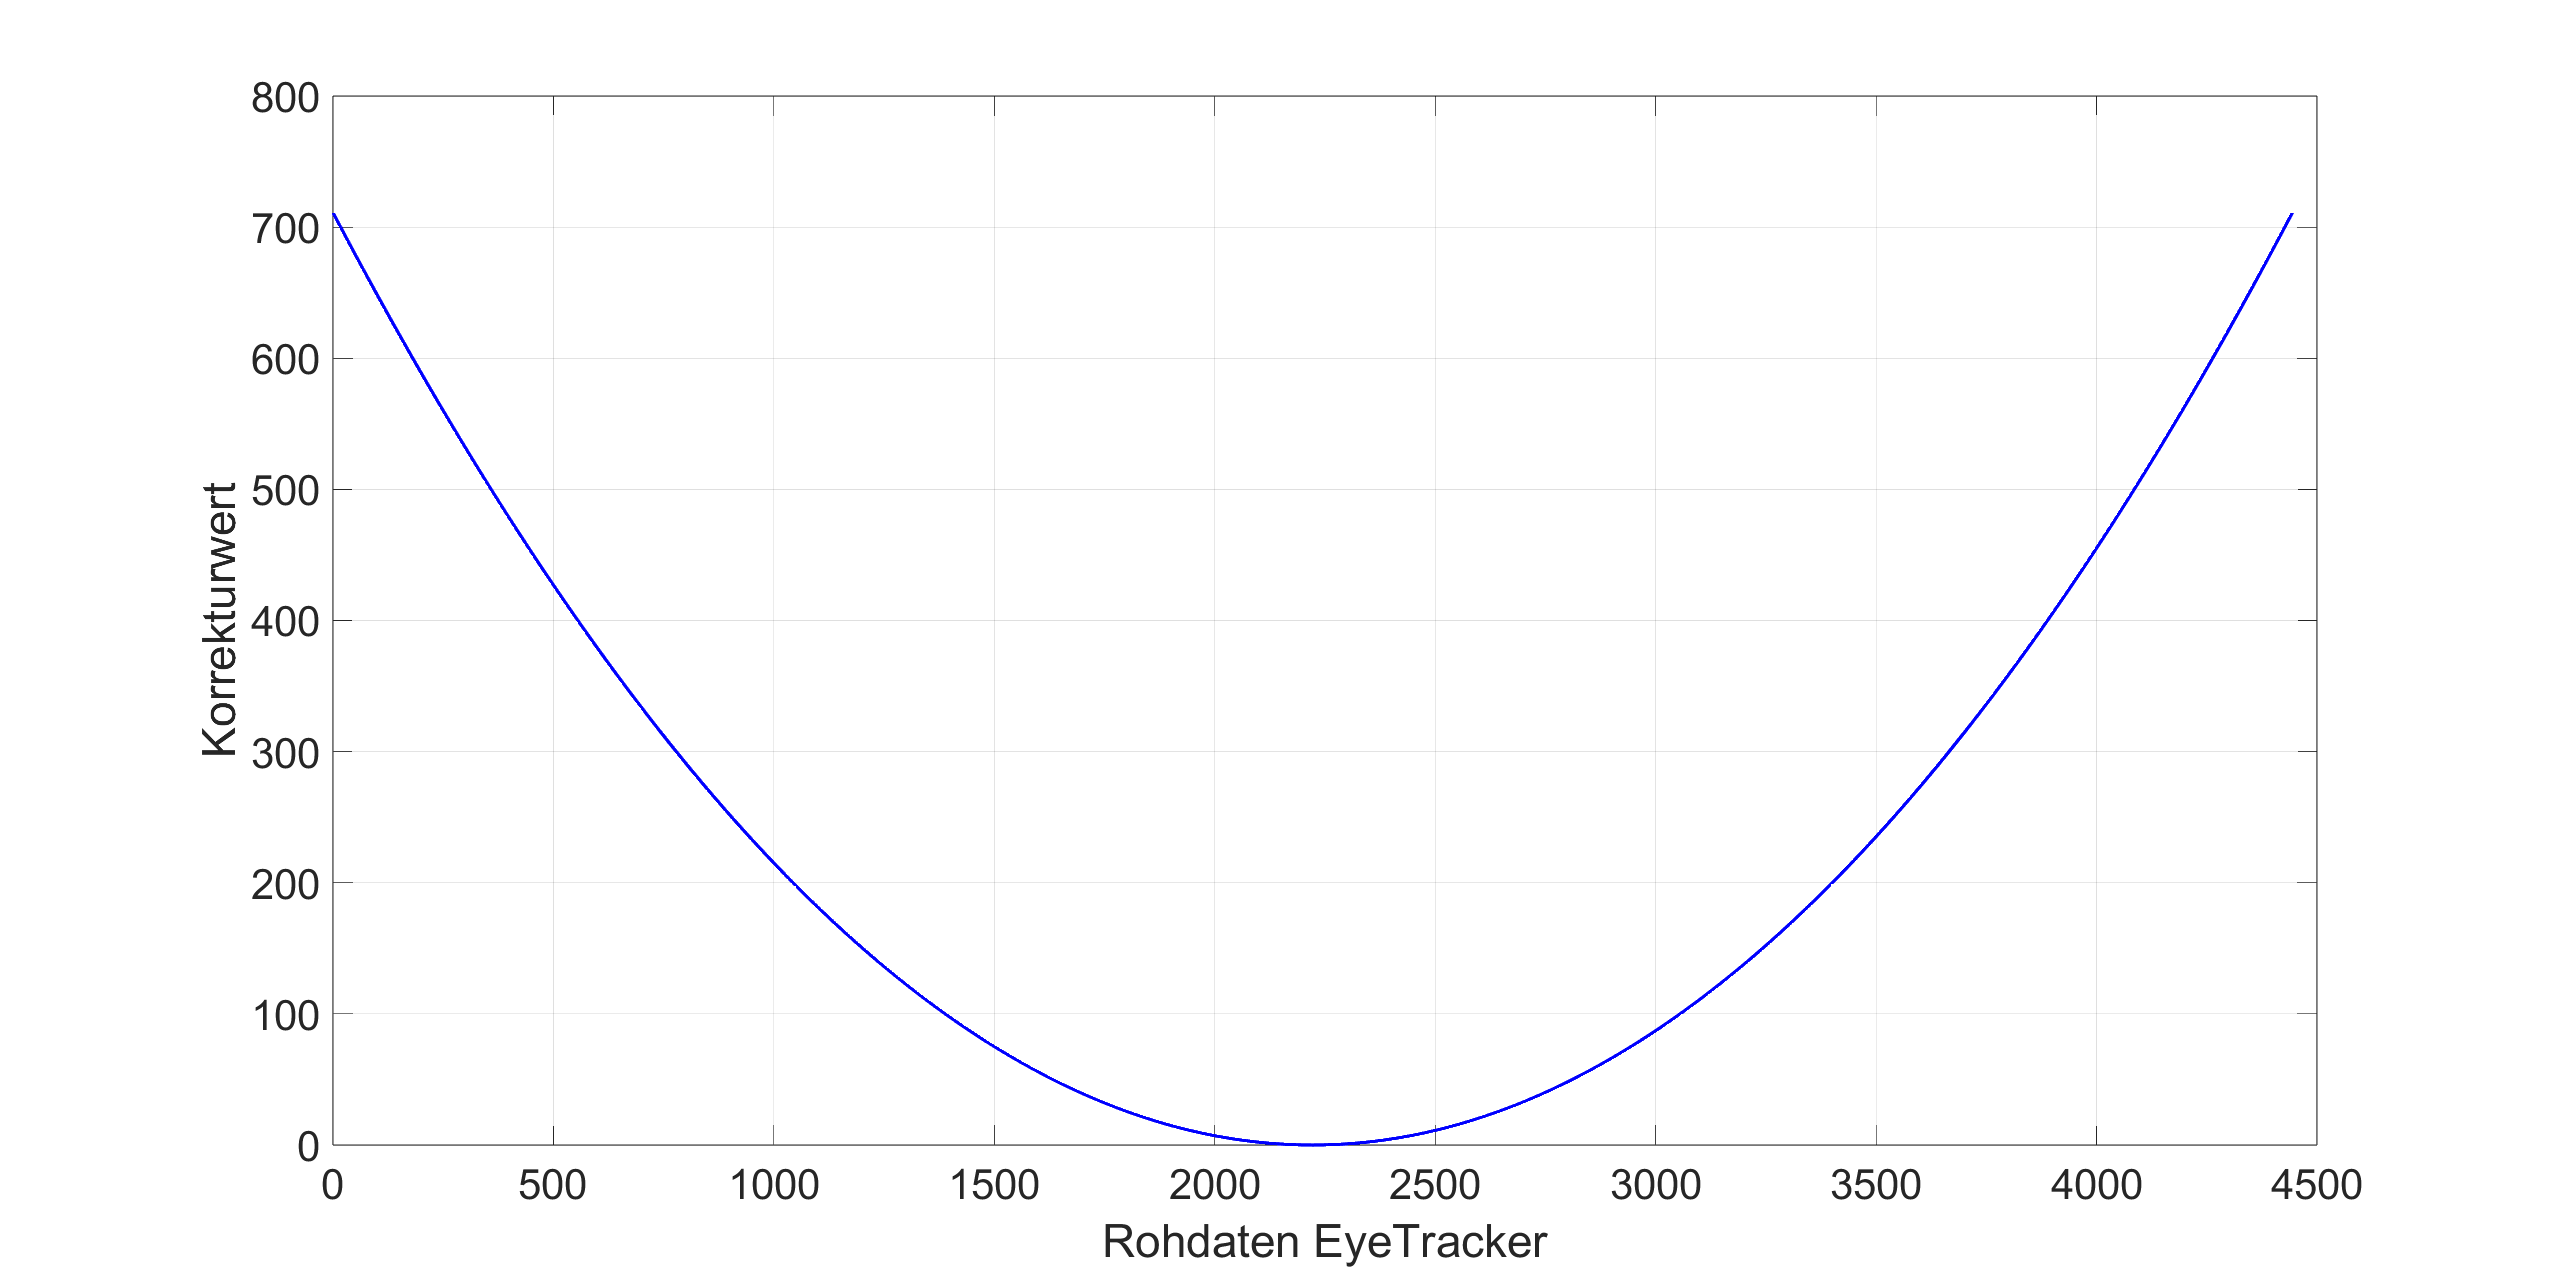
\includegraphics[scale=0.17]{first_correction_function_initialparam}
\caption{Visualisierung quadratische Korrekturfunktion, Quelle: \cite{lit_software_matlab}} \label{fig:imag8}
\end{center}
\end{figure}

Wie in Abbildung \ref{fig:imag8} zu erkennen ist, besteht jetzt im Vergleich zur e-Funktion eine stärkere Korrektur in der Nähe der Mitte der Leinwand. An den Rändern ist der Korrekturwert nicht so hoch wie bei der e-Funktion, wodurch der nutzbare Sichtbereich weniger stark eingeschränkt wird. 

Im Fahrsimulator war eine leichte Verbesserung spürbar und es wurde eine Auswertung der Ergebnisse durchgeführt. 

\begin{figure}[h!]
\begin{center}
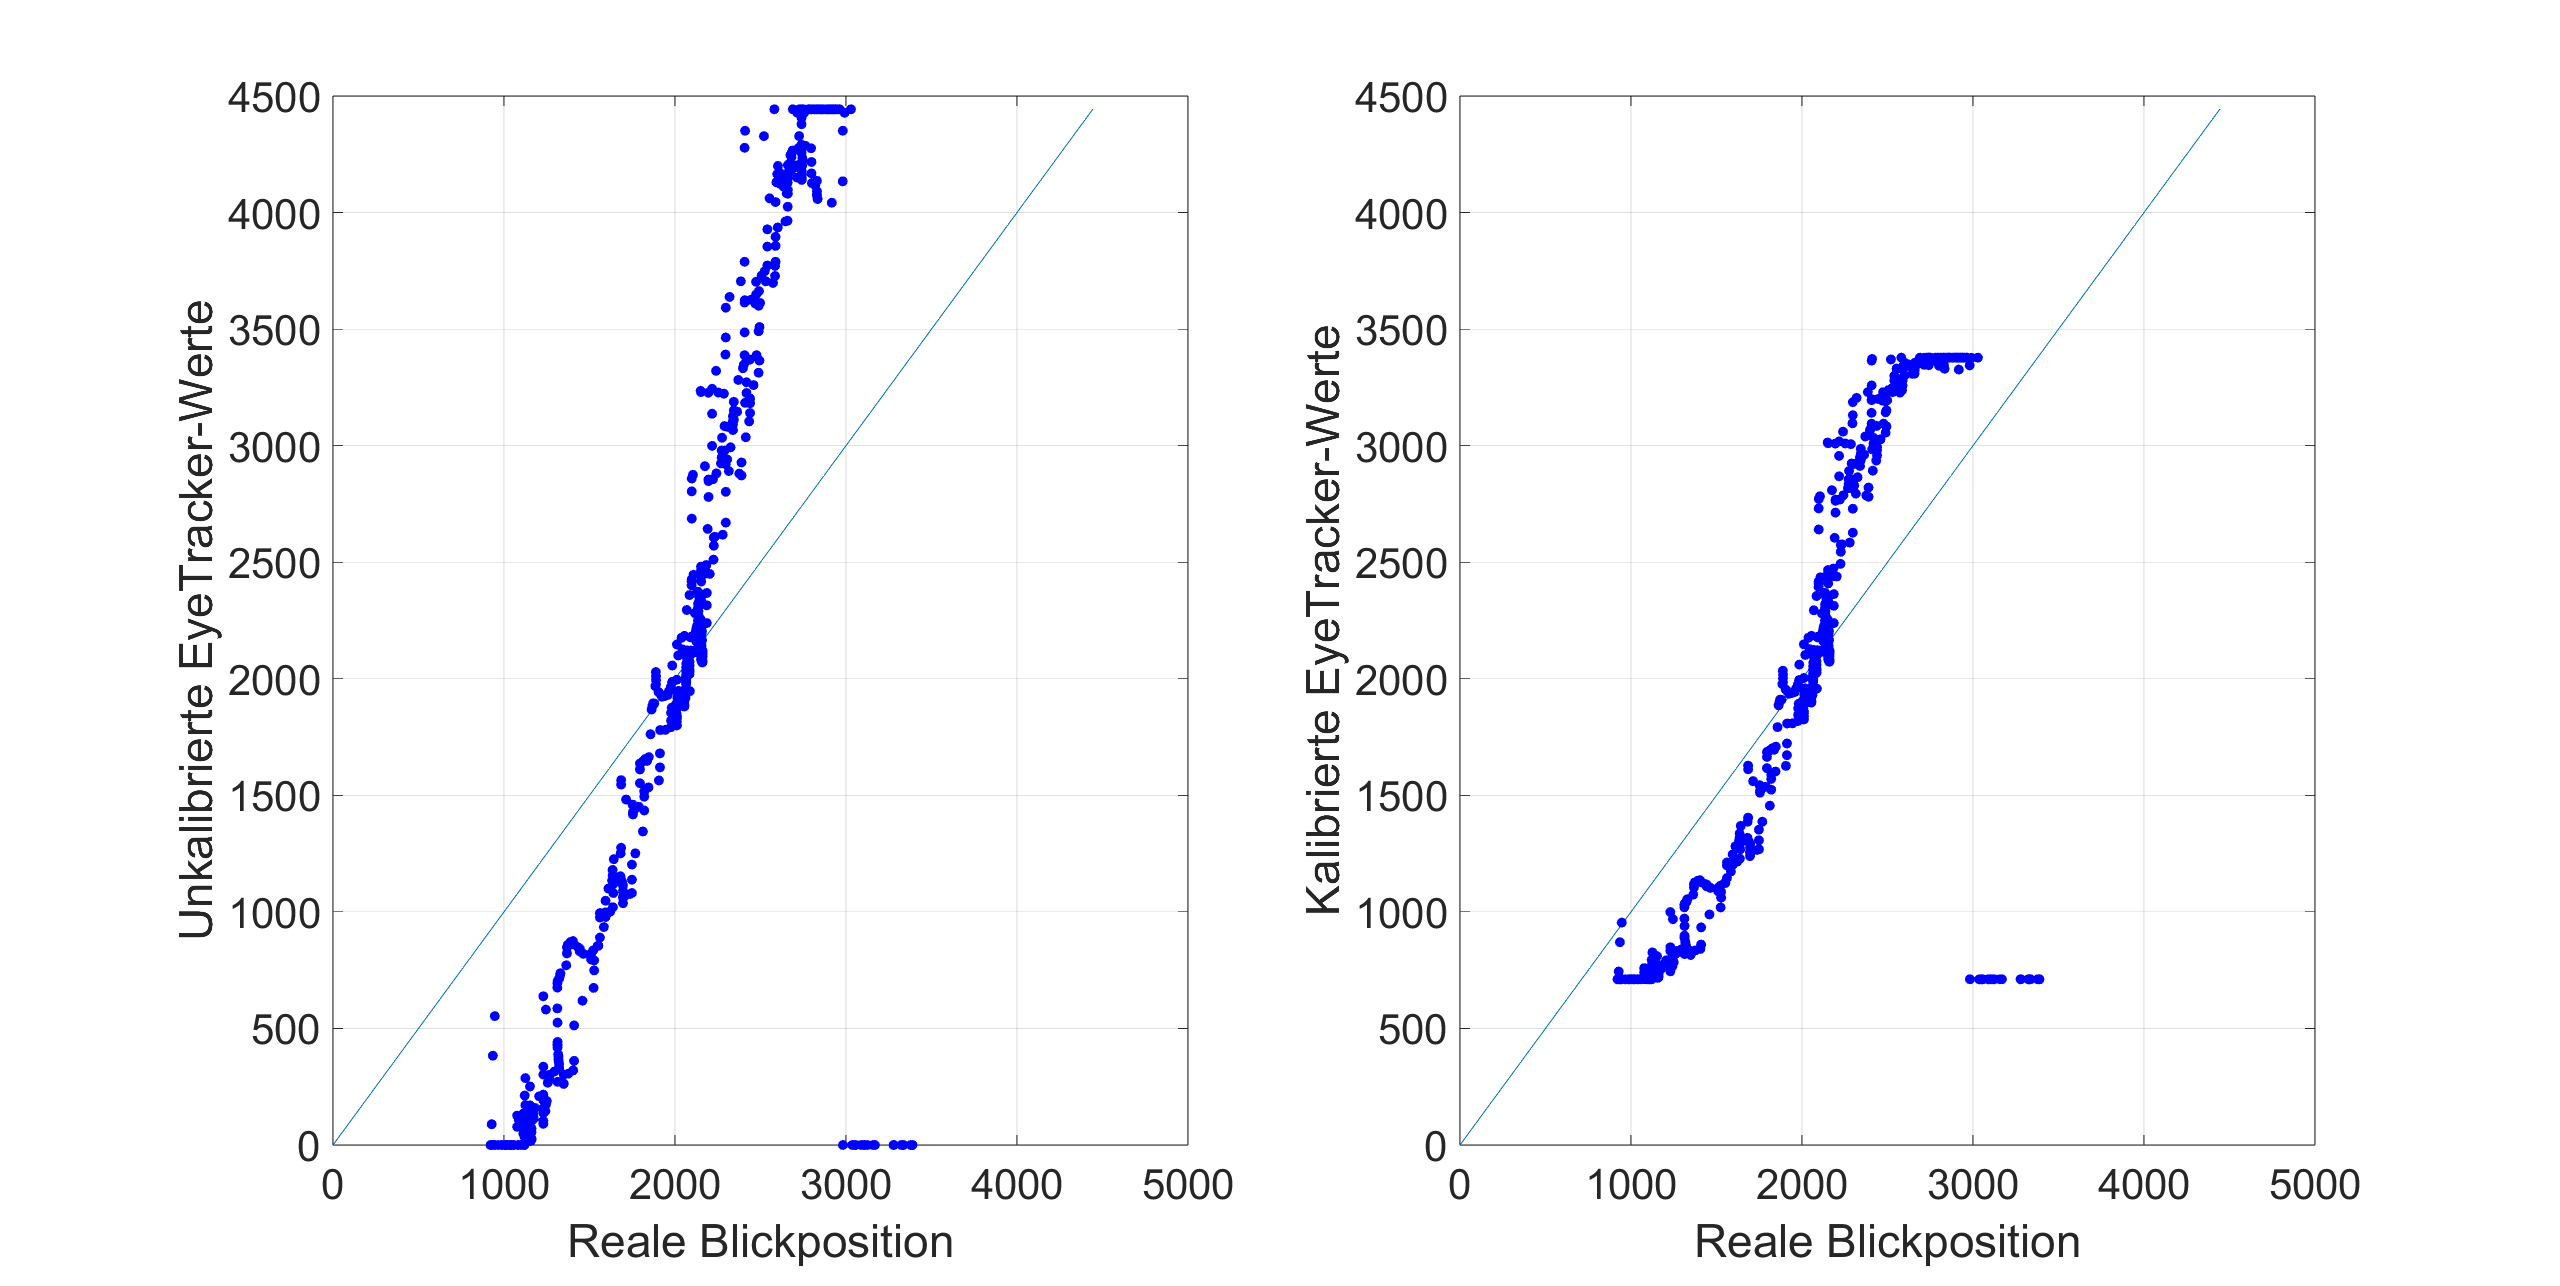
\includegraphics[scale=0.19]{first_correction_function_results}
\caption{Gegenüberstellung reale Blickposition und Eye Tracker-Werte: unkalibriert (links), kalibriert (rechts), Quelle: \cite{lit_software_matlab}} \label{fig:imag9}
\end{center}
\end{figure}

In Abbildung \ref{fig:imag9} sind die Ergebnisse zu erkennen. Auf der x-Achse ist die reale Blickposition in Pixel aufgetragen. Dabei entspricht 0 Pixel dem linken Bildschirmrand und 4444 Pixel dem rechten Bildschirmrand. Die reale Blickposition wurde mithilfe des Mauszeigers ermittelt. Die Testperson hat den Mauszeiger über den Bildschirm bewegt und ihn mit den Augen verfolgt.
Auf der y-Achse ist die vom Eye Tracker geschätzte Blickposition aufgetragen. Diese ist zur Vergleichbarkeit ebenfalls in Pixel angegeben. Für beide Graphen in Abbildung \ref{fig:imag9} werden auf der x-Achse dieselben Werte verwendet. Auf der y-Achse werden beim linken Graphen die Rohdaten des Eye Trackers aufgetragen. Beim rechten Graphen werden die von unserer quadratischen Funktion kalibrierten Werte angezeigt. Im Idealfall sollten die blauen Punkte deckungsgleich mit der hellblauen monoton steigenden Gerade sein. Um zu prüfen, dass unsere Kalibrierung gut funktioniert, sollten die blauen Punkte im rechten Graphen zum einen so nahe wie möglich an der blauen Gerade anliegen und zum anderen bessere Ergebnisse als im linken Graphen erzielt werden. 

Es ist zu erkennen, dass der Sichtbereich auch bei der Verwendung einer quadratischen Korrekturfunktion eingeschränkt wird. Diese Einschränkung konnte allerdings reduziert werden. Bei der e-Funktion war der maximale Korrekturwert auf der linken Bildschirmhälfte k=1300. Bei der abgestimmten, quadratischen Korrekturfunktion liegt das Maximum bei k=700. Es stehen somit auf der linken Bildschirmhälfte 600 Pixel mehr für das Tracking zur Verfügung. Die Auswertung stimmt mit den theoretischen Überlegungen soweit überein, dass bei ca. 2222 Pixel ein Fehler von null vorhanden ist. Das liegt daran, weil die gekrümmte Leinwand und eine äquivalente, imaginäre, gerade Leinwand in der Bildschirmmitte bei 2222 Pixel identisch sind. 
Um die Verbesserungen deutlich zu erkennen, müssen bestimmte Bereiche genauer betrachtet werden: 


\begin{figure}[h!]
\begin{center}
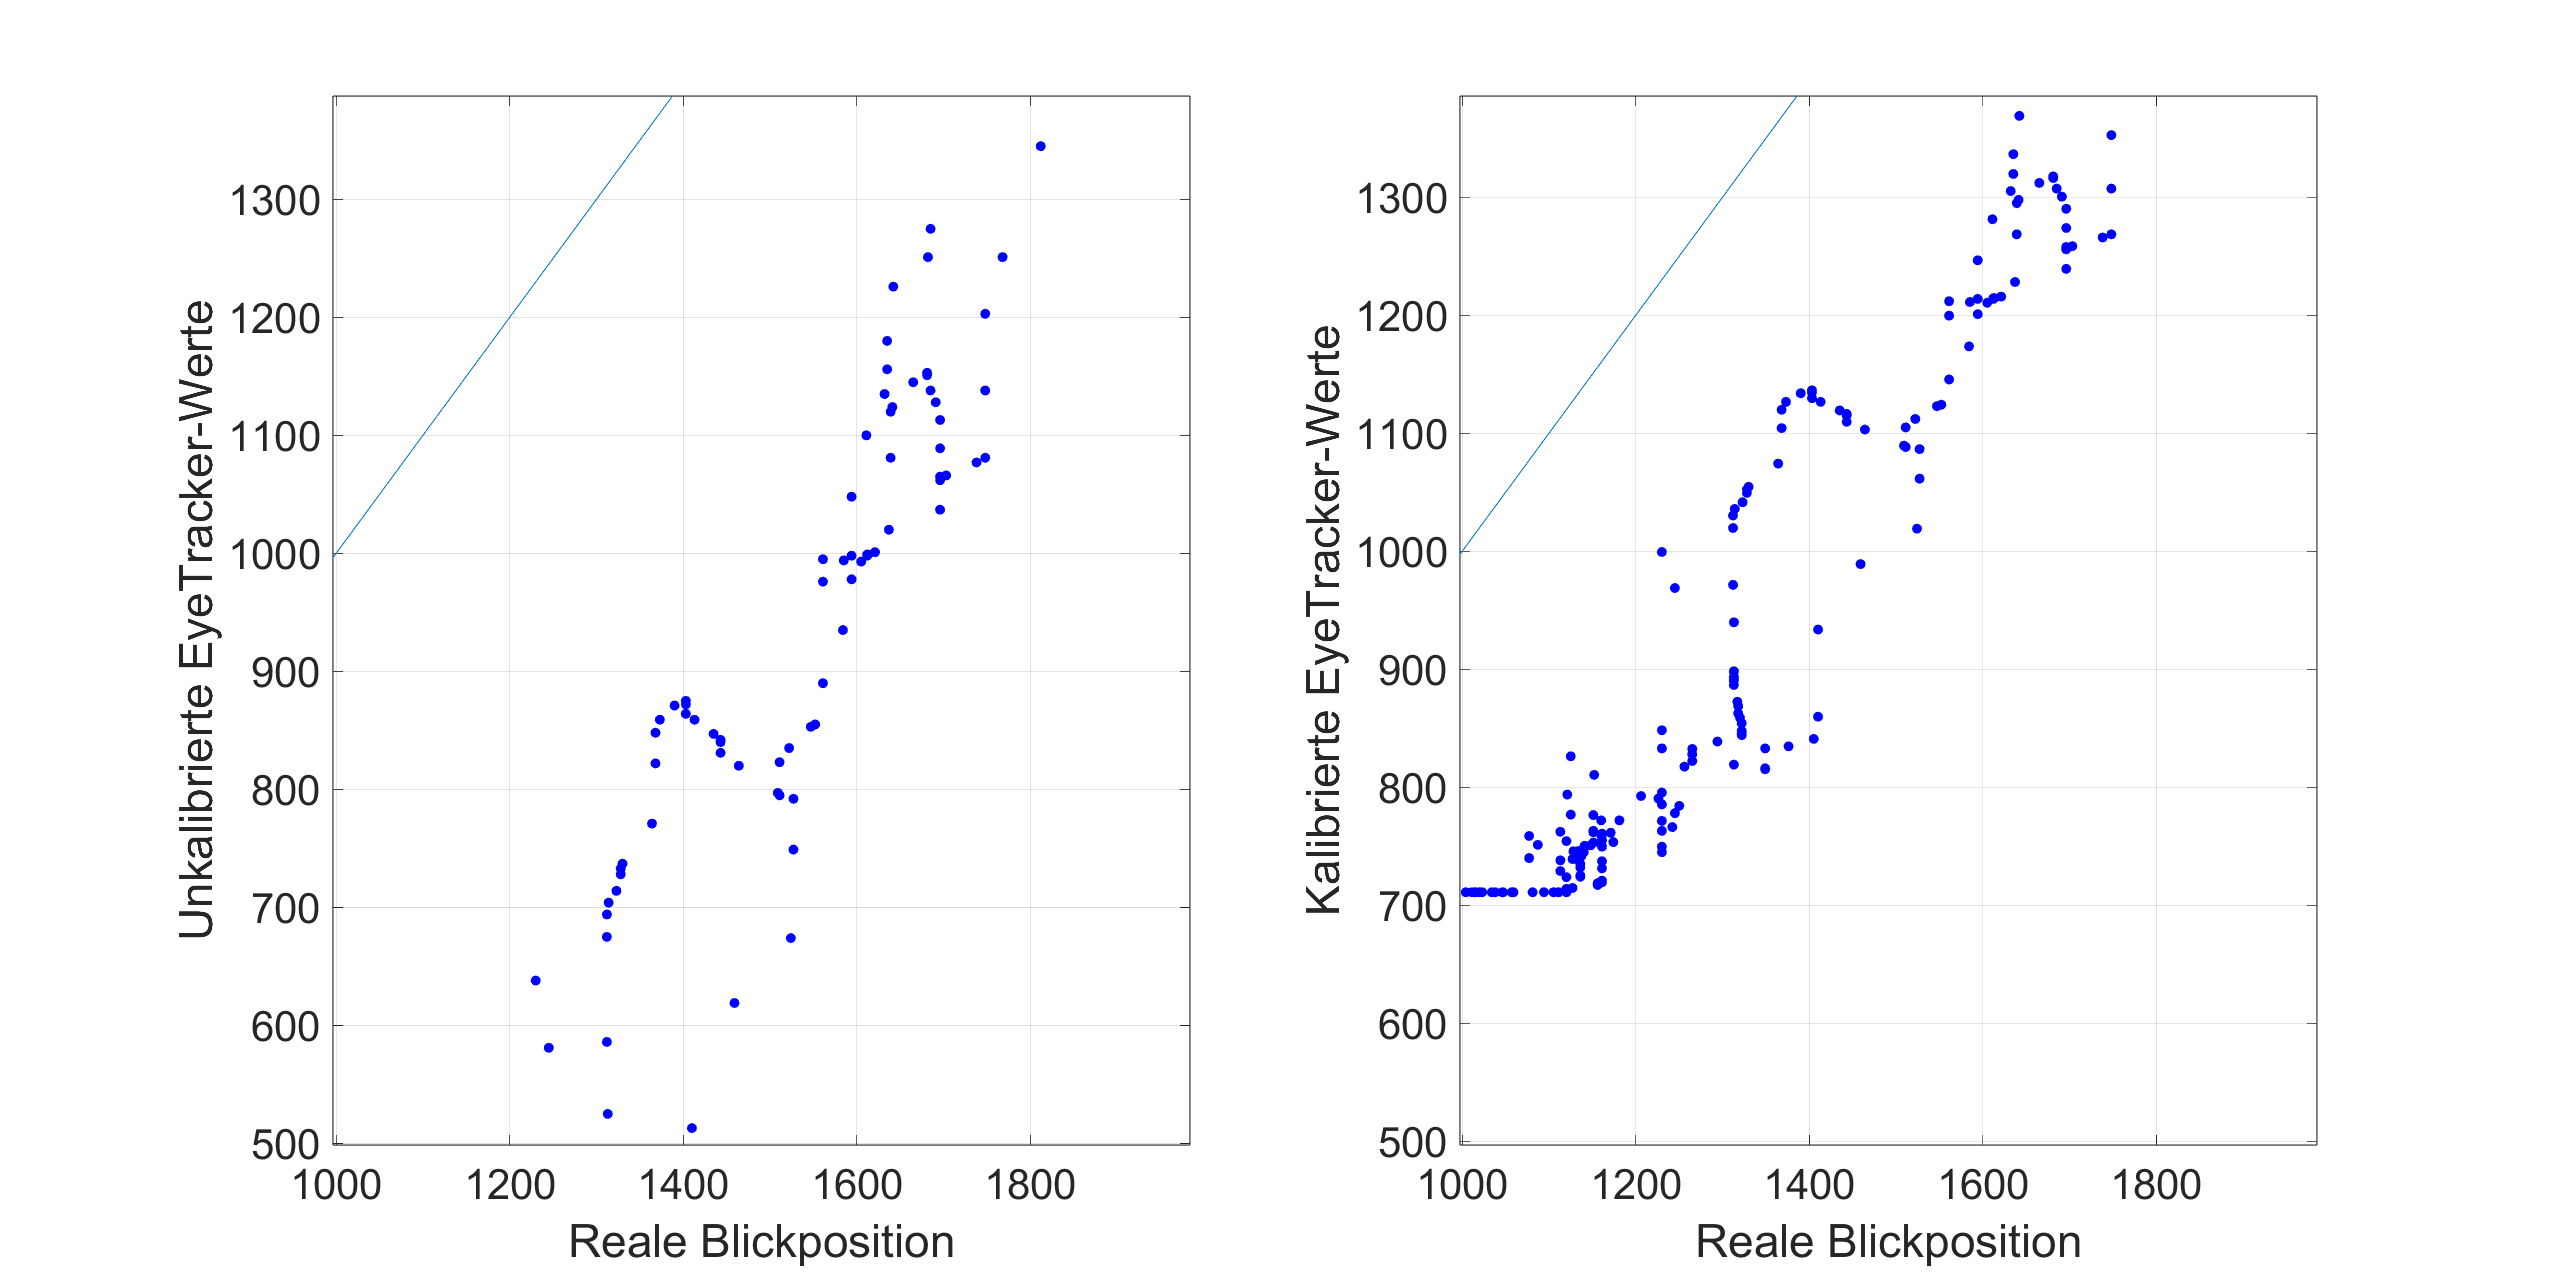
\includegraphics[scale=0.19]{first_correction_function_results_zoomed}
\caption{Gegenüberstellung reale Blickposition und Eye Tracker-Werte im Detail: unkalibriert (links), kalibriert (rechts), Quelle: \cite{lit_software_matlab}} \label{fig:imag10}
\end{center}
\end{figure}

In Abbildung \ref{fig:imag10} ist ein Detail-Ausschnitt der Ergebnisse der linken Leinwand-Hälfte zu erkennen. Es ist deutlich zu sehen, dass die Werte nach der Kalibrierung näher an der idealen Geraden liegen. Je näher sich die Blickposition dem linken Bildschirmrand näher, umso geringer wird der absolute Fehler. Es ist allerdings auch festzustellen, dass in Richtung Bildschirmmitte weiterhin zu wenig korrigiert wird. Dort ist generell ein geringer Fehler zwischen gekrümmter und gerade Leinwand zu erwarten. Dennoch ist der dort fast so hoch wie in Randnähe. Würde der Parameter c erhöht werden, dann würde der Fehler reduziert werden. Gleichzeitig würde allerdings auch der nutzbare Erfassungsbereich des Eye Trackers reduziert werden. Es bestehen dieselben Probleme wie bei der e-Funktion, nur weniger stark ausgeprägt. 

Eine Funktion 4. Grades scheint auf den ersten Blick sinnvoll. Diese steigt zwar stärker an als eine quadratische Funktion, allerdings besitzt sie in ihrem Ursprung ein Plateau. Dadurch wäre die Korrektur im Bereich der Bildschirmmitte definitiv nicht ausreichend. 


\subsubsection{V-Funktion mit abgeflachtem Beginn und Ende}

Nach den Experimenten im Fahrsimulator wurde aus den daraus gewonnen Erfahrungen eine Funktion gesucht, welche in der Bildschirmmitte einen Korrekturwert von null ausgibt. Die Funktion sollte einen Korrekturfaktor ausgeben, welcher sich relativ zum Abstand zu der Bildschirmmitte erhöht. Dabei sollte dieser Anstieg bereits unmittelbar um die Bildschirmmitte hoch sein, damit der Fehler dort bereits ausreichend verringert wird. An den Rändern soll sie allerdings nicht zu sehr ansteigen, da sonst der nutzbare Sichtbereich reduziert werden würde. Als Kurvendiagramm sollte die Funktion wie ein V aussehen, dessen Tiefpunkt auf der x-Achse bei der Bildschirmmitte, also bei 2222 Pixeln liegt. In Richtung der Ränder sollte die Steigung der Funktion kleiner werden, damit der nutzbare Sichtbereich des Eye Trackers nicht zu sehr eingeschränkt wird. Dieser sollte im Idealfall größer sein, als bei der quadratischen Funktion. 

Damit die Steigung stufenlos angepasst werden kann, wurde eine Variable p dafür verwendet. Damit keine negativen Werte herauskommen, muss mithilfe des Betrags sichergestellt werden, dass innerhalb der Basis keine negativen Werte vorkommen. Damit die V-Funktion ihren Tiefpunkt in der Bildschirmmitte hat, muss sie um die Bildschirmmitte nach rechts verschoben werden:

\begin{equation} \label{eq:5}
	k=|x-w|^p
\end{equation}

Zusätzlich wird der Faktor c eingeführt, welcher ähnlich wie p die Steigung relativ zum Abstand zur Bildschirmmitte beeinflusst. Allerdings nicht ganz so aggressiv wie p. Ein Parameter d wurde eingeführt, um ein Grund-Offset zu erzeugen, welches bei der Feinabstimmung evtl. nützlich sein könnte. 

\begin{equation} \label{eq:6}
	k=(c*|(x-w)|+d)^p
\end{equation}

Damit sich die Ränder der Funktion gegen einen bestimmten Wert annähern, muss eine Dämpfung in die Funktion eingebaut werden. Diese wird durch eine e-Funktion realisiert. Dadurch ist eine schnelle Annäherung an den Grenzwert sichergestellt. Die vollständige Korrekturfaktor-Funktion ist wie folgt definiert: 


\begin{equation} \label{eq:6}
	k=(c*|(w-x)|+d)^p*(1-e^{-g*(|w-x|)})
\end{equation}



\begin{figure}[h!]
\begin{center}
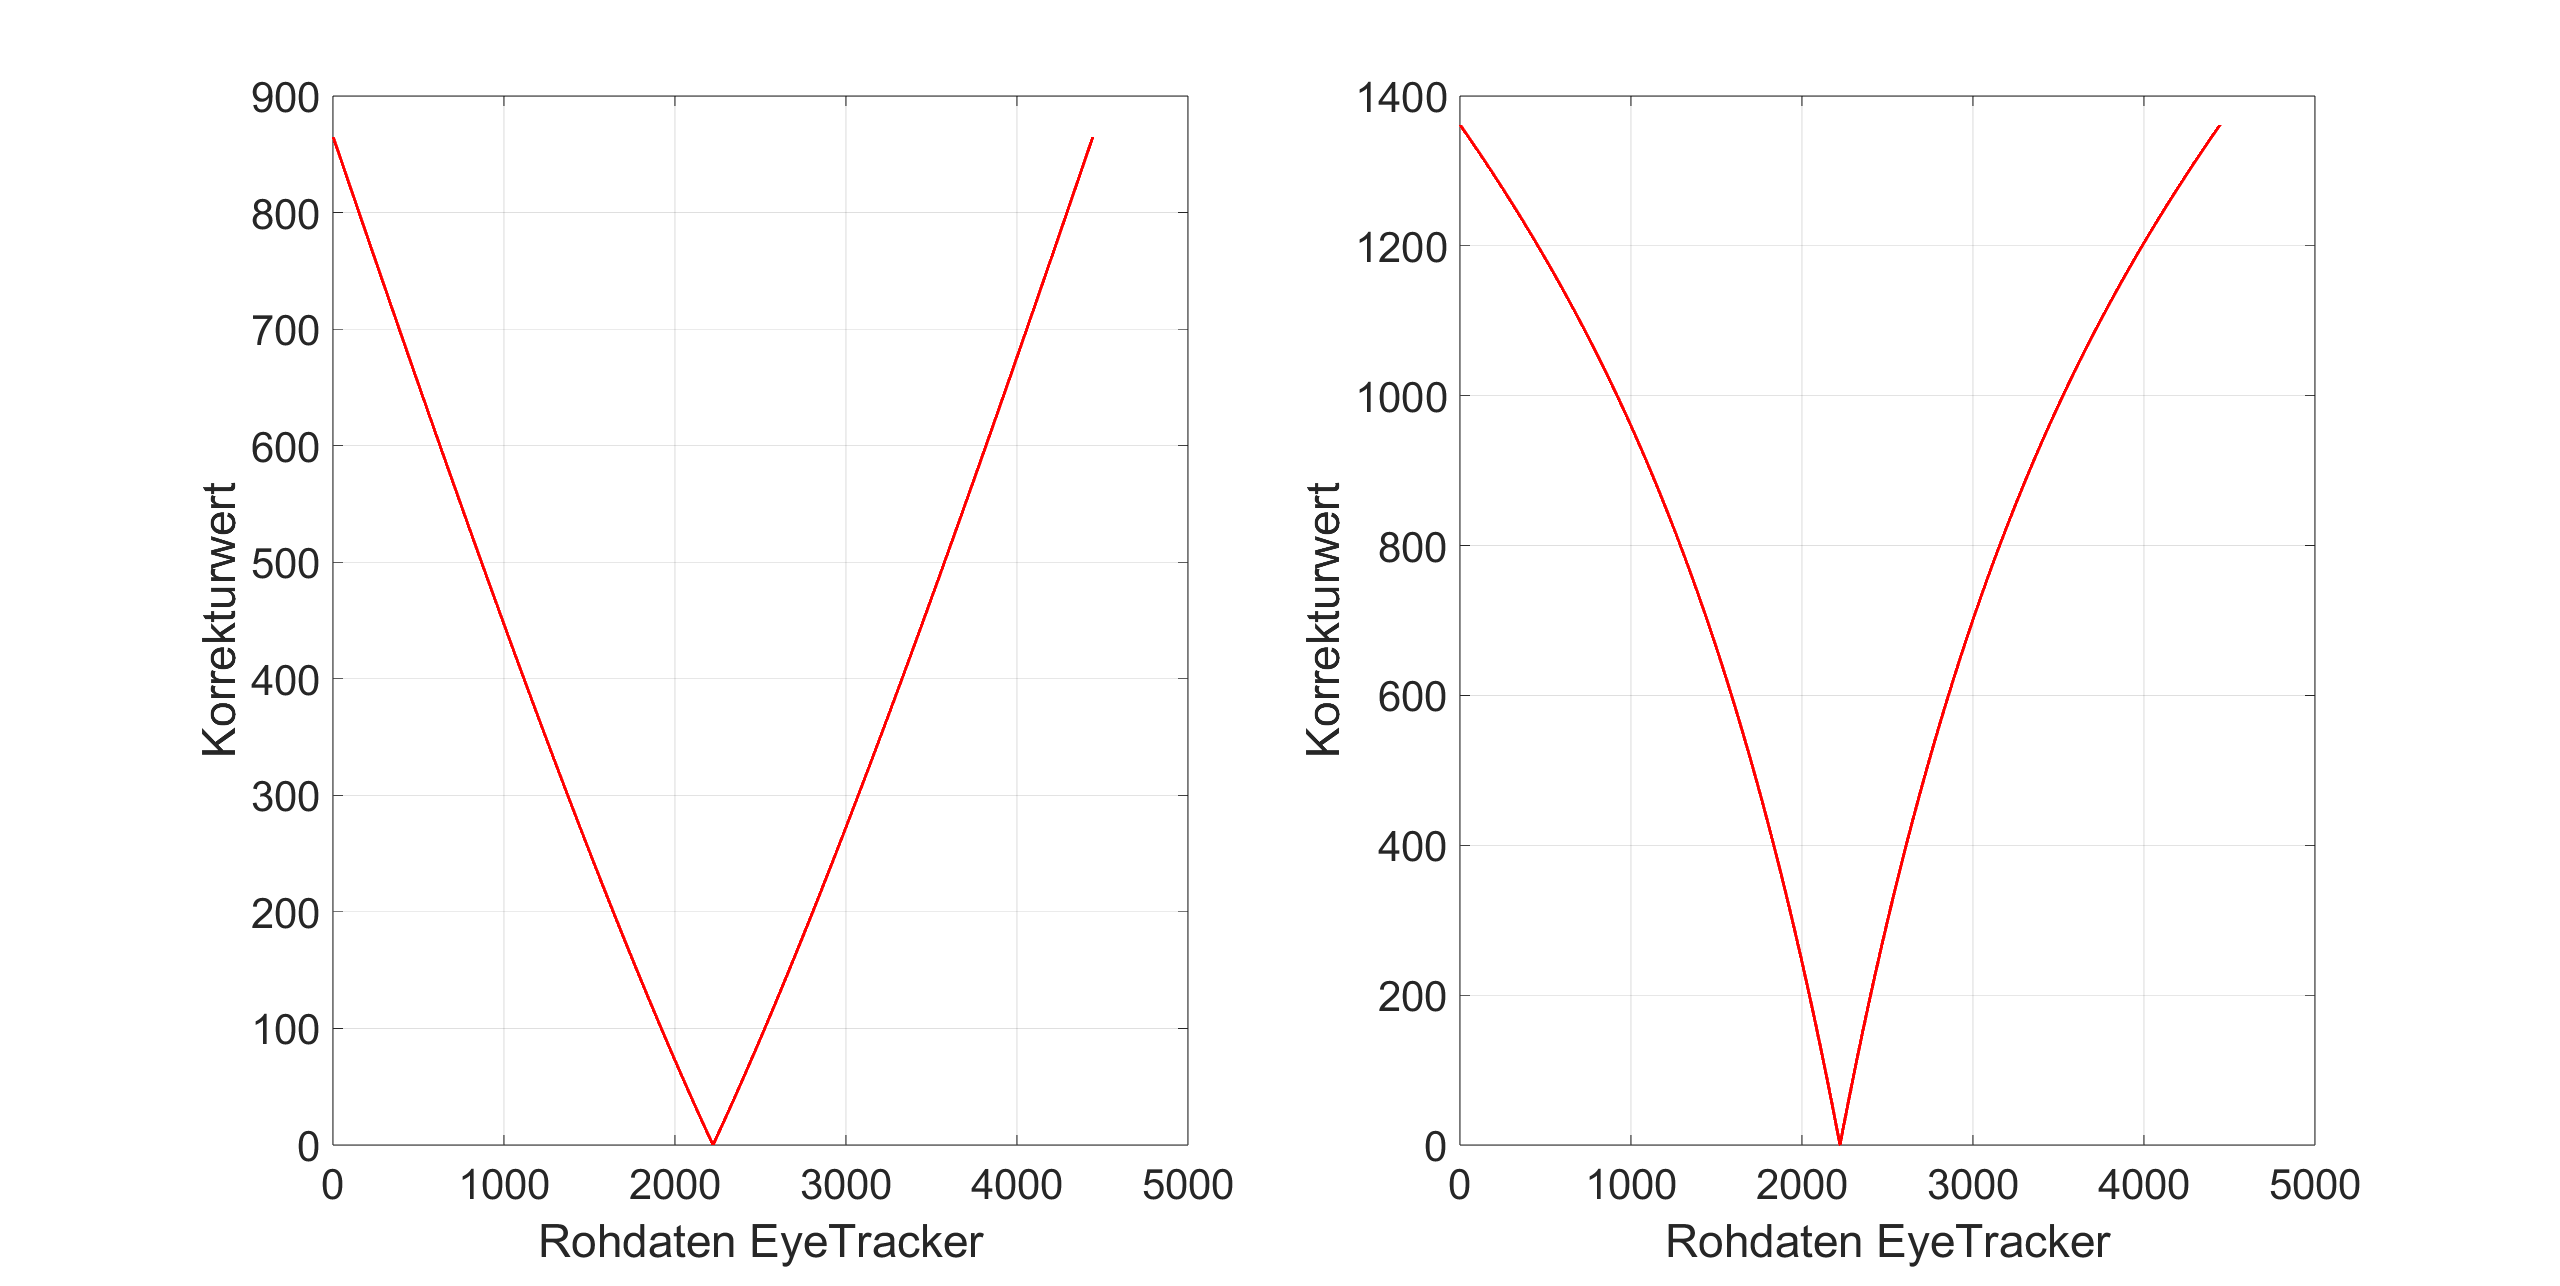
\includegraphics[scale=0.19]{second_correction_function_param}
\caption{Korrekturfunktion: linke Bildschirmhälfte (links), rechte Bildschirmhälfte (rechts), Quelle: \cite{lit_software_matlab}} \label{fig:imag11}
\end{center}
\end{figure}


Die graphische Darstellung der Korrekturfunktion ist in Abbildung \ref{fig:imag11} zu erkennen. Die optimalen Parameter wurden im Fahrsimulator experimentell bestimmt und werden für die Darstellung des Graphen verwendet. Wie in der Abbildung zu erkennen ist, unterschieden sich die Parameter zwischen linker und rechter Leinwandhälfte. Auf der rechten Hälfte muss stärker korrigiert werden. Hier ist die Veränderung der Steigung ab einem gewissen Punkt gut zu erkennen. 

\begin{figure}[h!]
\begin{center}
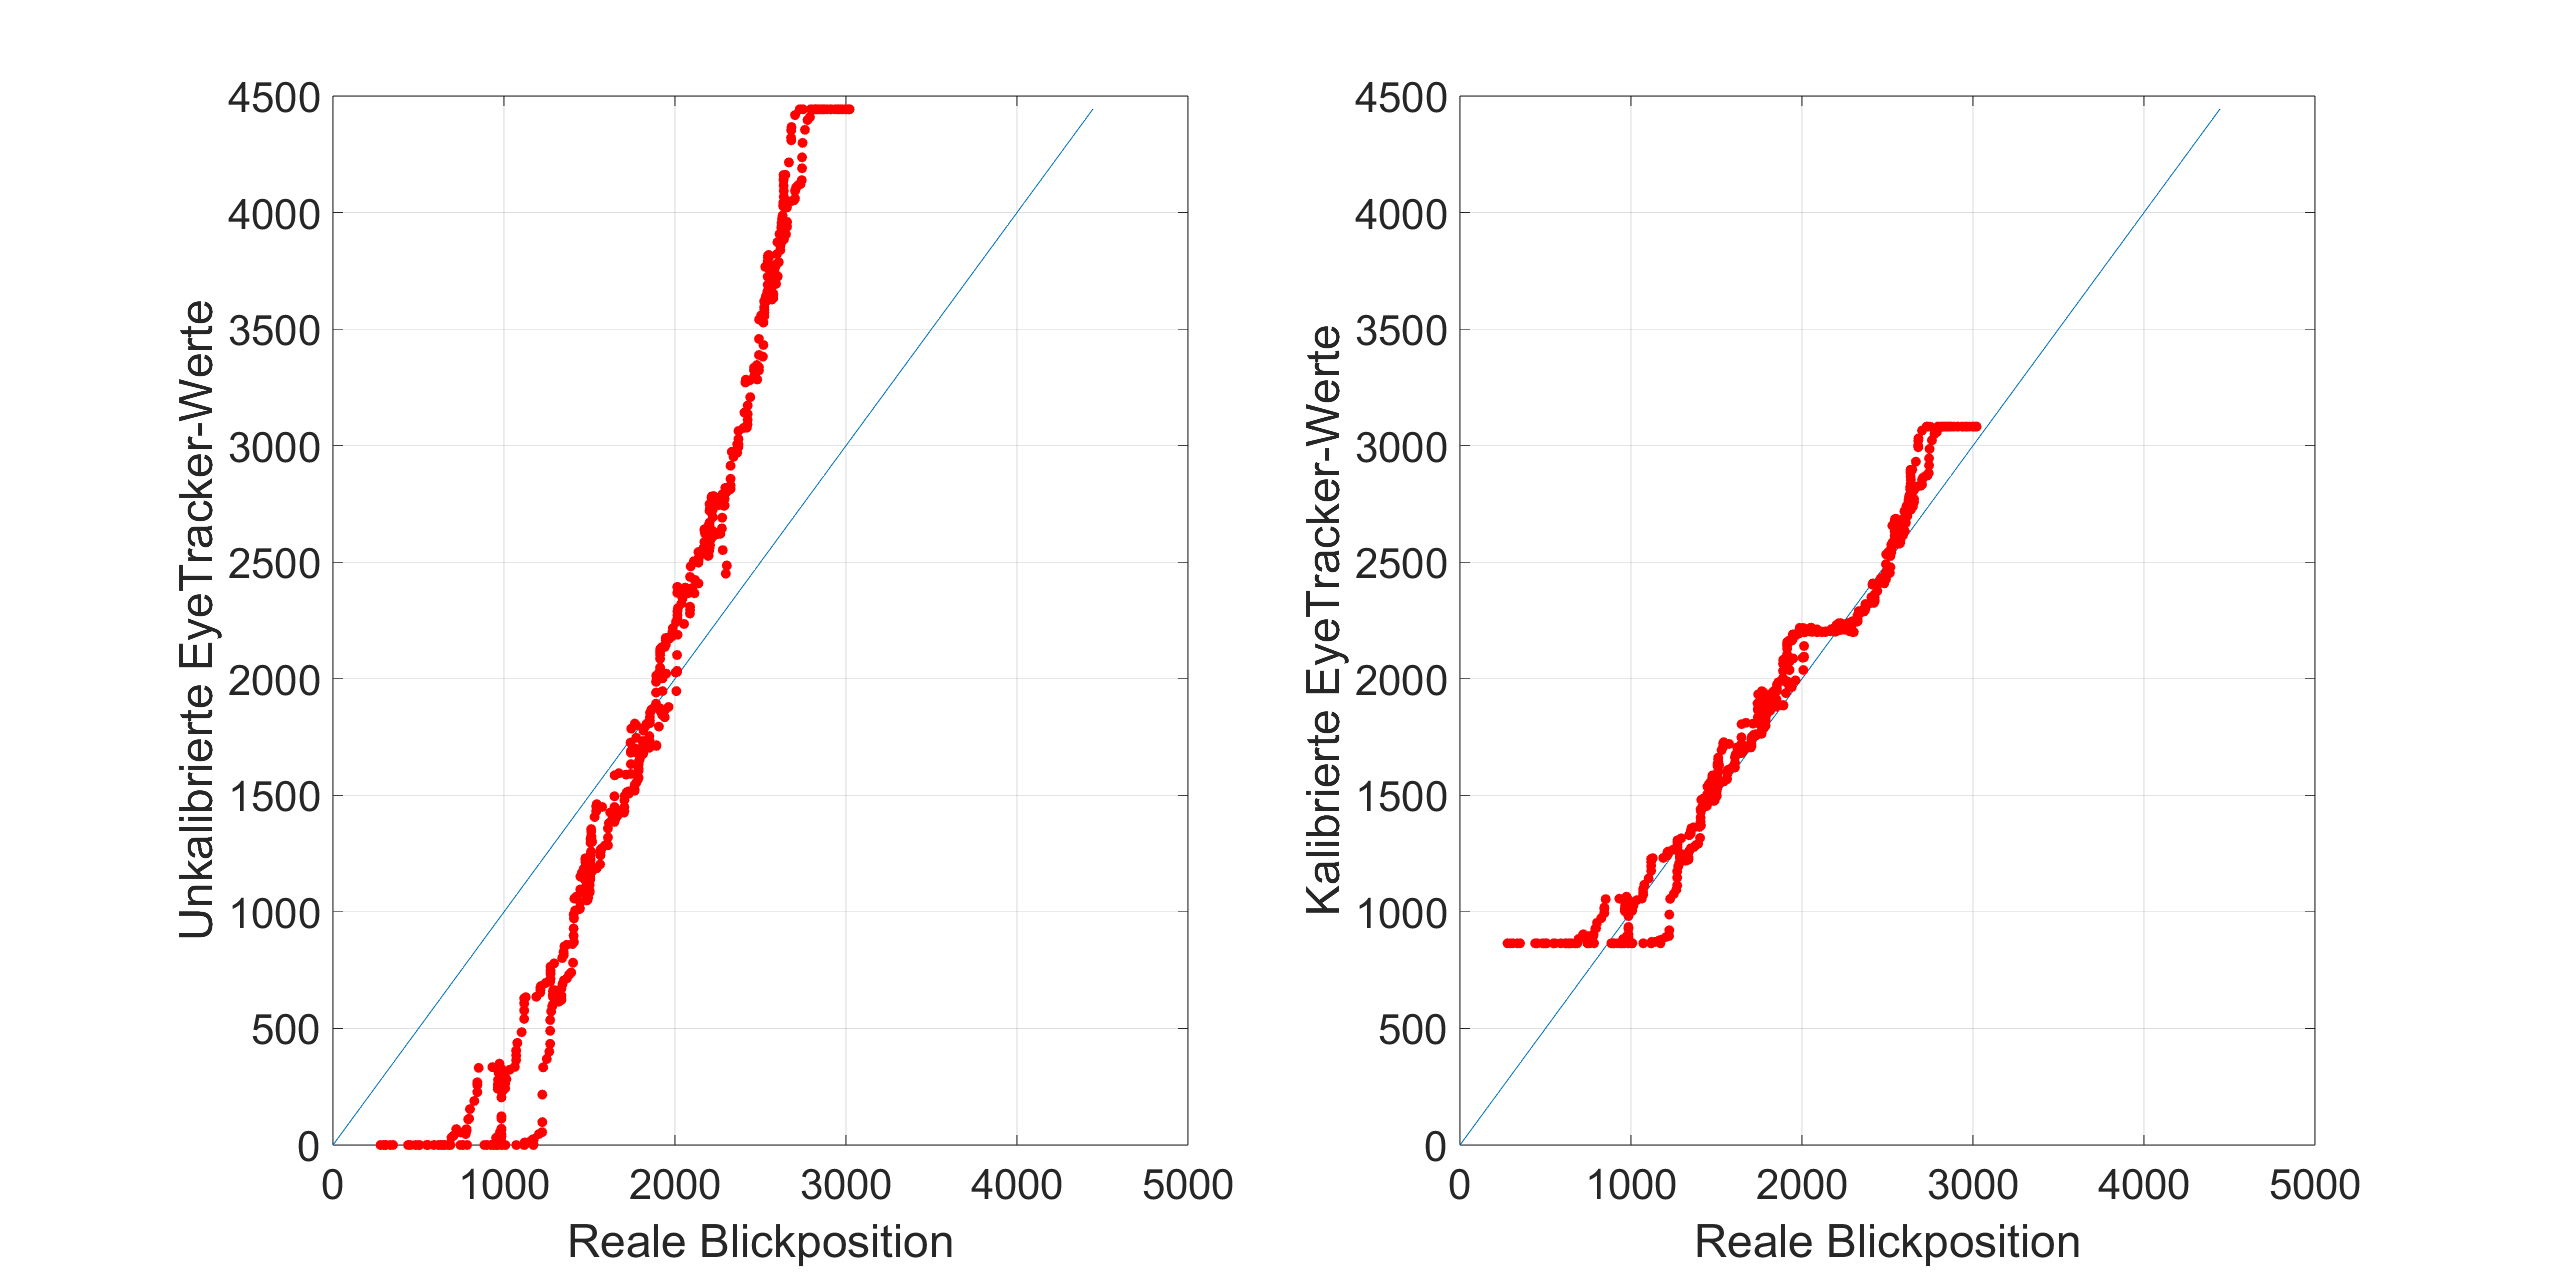
\includegraphics[scale=0.19]{second_correction_function_results}
\caption{Gegenüberstellung reale Blickposition und Eye Tracker-Werte: unkalibriert (links), kalibriert (rechts), Quelle: \cite{lit_software_matlab}} \label{fig:imag12}
\end{center}
\end{figure}

In Abbildung \ref{fig:imag12} sind die Ergebnisse zu erkennen, welche mit der neuen v-förmigen Korrekturfunktion erzielt werden konnten. Es ist eine deutliche Verbesserung gegenüber der quadratischen Korrekturfunktion zu erkennen. Ein eingeschränkter Sichtbereich ist weiter vorhanden. Da ab einem gewissen Punkt allerdings sowieso keine verwertbaren Werte mehr geliefert werden ist das nicht problematisch. Der Eye Tracker korrigiert in der Nähe der Bildschirmmitte jetzt aggressiver und hat damit Erfolg. Auch in Randnähe wieder stärker korrigiert und somit der Fehler reduziert. Durch die unterschiedlichen Parameter für linke und rechte Bildschirmhälfte entsteht im Übergang von linker auf rechte Bildschirmhälfte und anders herum ein kleiner Sprung. Eine weitere Optimierung würde den Rahmen dieser Projektarbeit übersteigen.



\begin{figure}[h!]
\begin{center}
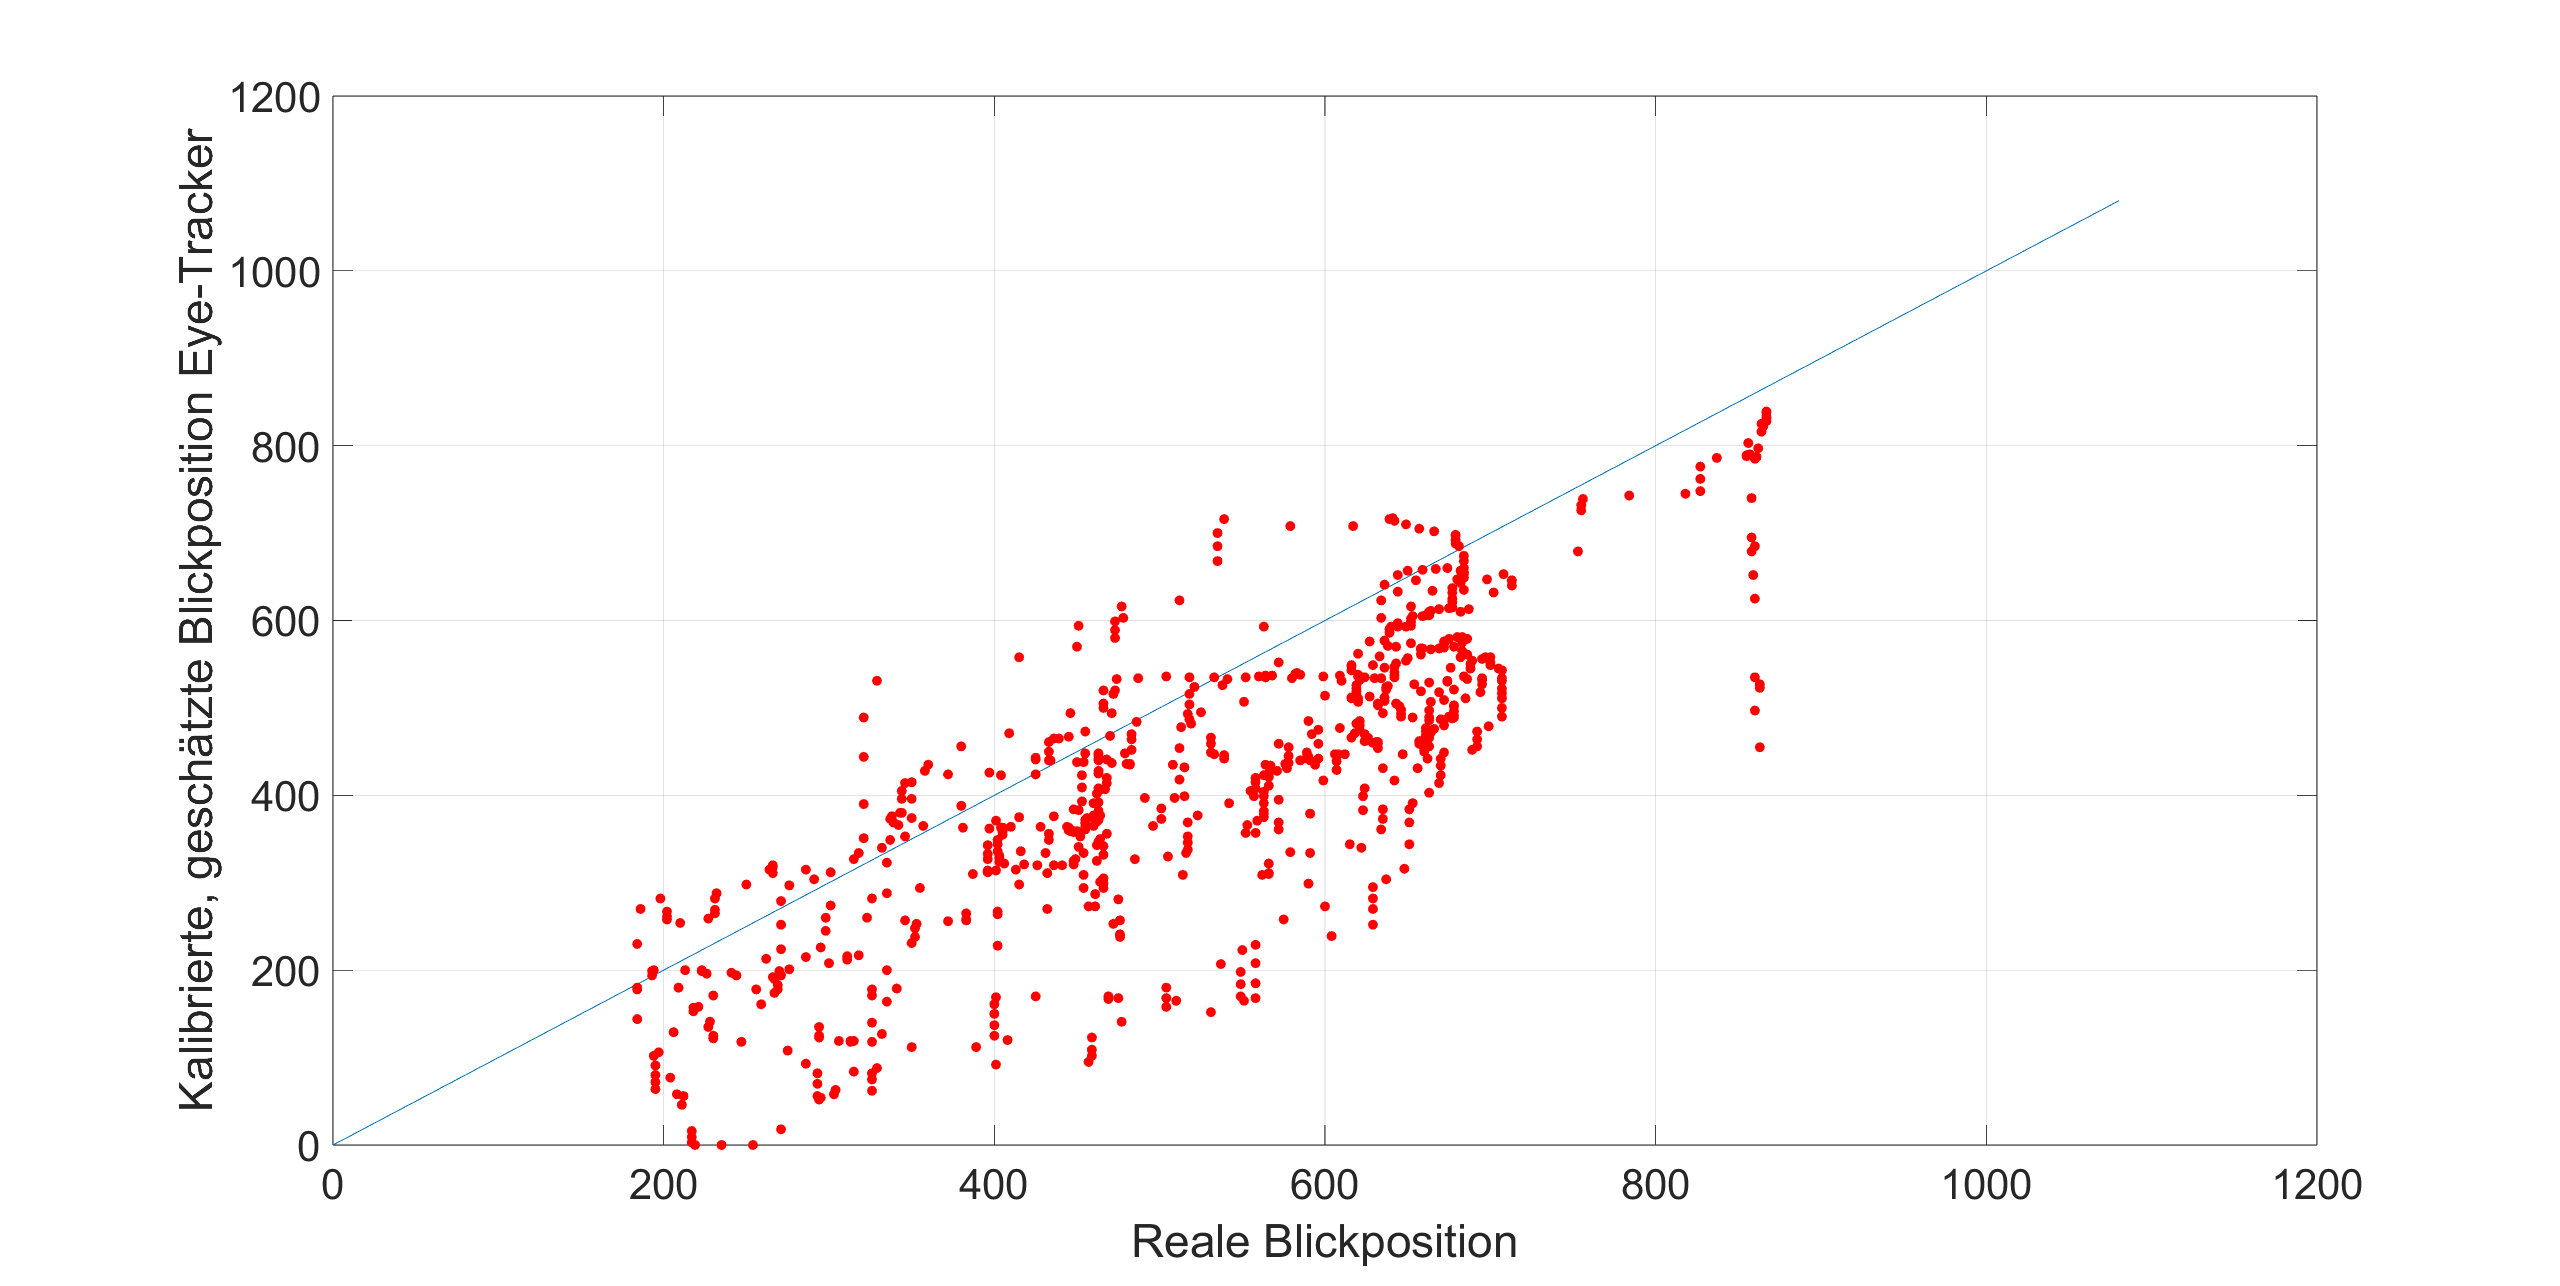
\includegraphics[scale=0.19]{second_correction_function_results_y}
\caption{Gegenüberstellung reale Blickposition und Eye Tracker-Werte y-Achse kalibriert, Quelle: \cite{lit_software_matlab}} \label{fig:imag13}
\end{center}
\end{figure}

In Abbildung \ref{fig:imag13} ist die Auswertung der y-Achse nach der Kalibrierung dargestellt. Auf den ersten Blick wirkt es so, als wären die Tracking Ergebnisse auf der y-Achse schlechter als auf der x-Achse. Das liegt allerdings zum Teil an der anderen Skalierung der y-Achse im Diagramm. Bei den horizontalen Pixelwerten in den Abbildungen weiter oben war die y-Achse von null bis 4444 skaliert. Die y-Achse für die vertikalen Pixelwerte ist allerdings nur von null bis 1080 skaliert. Eine Abweichungen von bspw. 300 Pixeln wirkt im Graphen für die vertikalen Pixel größer als im Graphen für horizontale Pixel. Ein anderer Grund ist, dass keinerlei Optimierung der vertikalen Pixel durch unseren Code vorgenommen wird. Für die Optimierung der horizontalen Pixel durch die Krümmung der Leinwand wurden große Aufwände betrieben. Durch eine Optimierung der vertikalen Pixel könnten evtl. noch weitere Verbesserungen erzielt werden.




Eine abschließende Auswertung der Ergebnisse folgt in einem späteren Abschnitt.  





\section{Fazit}
\subsection{Auswertung und Zusammenfassung}

Alle Punkte aus der Zielsetzungen konnten im Rahmen der Projektarbeit umgesetzt werden. Die Ergebnisse zeigen, dass es mit einfachen Mitteln wie einer USB-Webcam und sehr preiswerter Software möglich ist, bereits verwertbare Ergebnisse zu generieren. Ursprünglich war angedacht eine Open Source Lösung als Fundament für den Eye Tracker zu verwenden. Nach ausgiebiger Marktrecherche konnte ein passendes Softwarefundament ausfindig gemacht werden. Der Beam Eye Tracker ist zwar nicht Open Source aber die Daten die er durch seine \acrshort{api} bereitstellen kann, bieten genug Spielraum, um individuelle Lösungen damit bauen zu können. Eine Verschmelzung zwischen Carla und dem Eye Tracker war ohne größeren Hürden möglich. Die Daten aus dem Instance Segmentation Sensor können zusammen mit den Werten des Eye Trackers ausgewertet werden. Somit ist es möglich nicht nur die geschätzten Koordinaten des Eye Trackers auf der Leinwand auszugeben, sondern auch das betrachtete Objekt innerhalb der Carla Simulationsumgebung zu bestimmen.
Während der Implementierung des Eye Tracking Systems sind an manchen Stellen auch Probleme aufgetreten. Die Belichtung war vor allem während der Kalibrierung ein Problem. Durch verschiedene Ansätze und Experimente im Fahrsimulator konnten hier mit externer Belichtung gute Ergebnisse erzielt werden.
Ein anderes Problem waren die verfälschten Tracking Daten, verursacht durch die gekrümmte Leinwand. Durch umfassende Analyse des Problems, einige mathematische Ansätze und Experimente im Fahrsimulator, konnte das Problem stark reduziert werden. Die in Abbildung \ref{fig:imag12} und \ref{fig:imag13} dargestellten Ergebnisse zeigen, dass gute Ergebnisse erzielt werden konnten. 
Die Tracking Daten sind allerdings nicht perfekt und lassen sich durch äußere Einflüsse wie schlechte Belichtung, Bedienungsfehler bei der Kalibrierung, Veränderung der Sitzposition nach der Kalibrierung oder zwei Personen gleichzeitig im Fahrsimulator negativ beeinflussen. Der Eye Tracker könnte allerdings zum aktuellen Entwicklungsstand bereits eingesetzt werden. Anhand der gemessenen Performance kann behauptet werden, dass bereits zum aktuellen Stand nützliche Erkenntnisse während einer Sitzung im Fahrsimulator mit einer Testperson gewonnen werden können. Im Ausblick sollen weitere Schritte und mögliche Ideen präsentiert werden, mit welchen über diesen Low Budget Ansatz hinaus, noch bessere Ergebnisse erzeugt werden könnten.


\subsection{Ausblick}

Angeknüpft an diese Projektarbeit kann eine Verbesserung des Testaufbaues erfolgen. Dazu zählen eine Ausbesserung der Lichtverhältnisse im Fahrsimulator, eine fest verbaute Kamera und gegebenfalls eine Blende, sodass nur der Fahrer von der Kamera erkannt wird. Ebenso kann die Eye Tracker Genauigkeit verbessert werden, indem die Korrektur für den gekrümmten Bildschirm durch einen Optimierungsalgorithmus ausgefeilt wird. Außerdem kann das Messergebnis durch eine Mittelwertsbildung der Pixelausgabe geglättet werden, um Messfehler in Echtzeit zu vermeiden. Eine Integration von künstlicher Intelligenz ist ebenfalls möglich.

Abschließend lassen sich weiterführende Analysen einbauen, wie die zeitliche Betrachtung von Blickpositionen und einer Aufbereitung der Blickposition in eine dreidimensionale Umgebung, sodass die Fahrt und die gemessene Blickposition anschaulich ausgewertet werden können.

\textcolor{red}{In den Anhang der Arbeit das Demo Video einfügen}

\clearpage

\printglossaries
\printbibliography


\end{document}
